\documentclass[a4paper]{article}
\usepackage[margin=3cm]{geometry}
\usepackage{xcolor}
\usepackage{graphicx}
\usepackage{lipsum}
\usepackage{amsmath}
\usepackage{pdfpages}
\usepackage{url}
%\usepackage[backref=page]{hyperref}
\usepackage{hyperref}
\usepackage{subcaption}
\usepackage[font=small,labelfont=bf]{caption}
\usepackage{siunitx}
\usepackage{circuitikz}
\hypersetup{
    colorlinks = true,
    colorlinks = false,
	urlcolor = {blue},
%	linkbordercolor = {transparent},
    pdfborder = {0 0 0},
	linkcolor = {blue},
	citecolor = {blue}
}
\usepackage{acronym}
\usepackage[acronym,nomain]{glossaries}
\makeglossaries
\newcommand{\todo}[1]{\textbf{\textcolor{red}{#1}}}
%\newcommand{\td}[1]{\textbf{\textcolor{red}{#1}}}
\newcommand{\td}[1]{\textcolor{red}{#1}}
\newcommand{\me}[1]{\textcolor{gray}{#1}}
\newcommand{\ds}[1]{}
\newcommand{\x}{$\times$}
\newcommand{\picwidth}{0.7\textwidth}

%SI UNITS
\newcommand{\cm}[1]{\SI{#1}{\centi\meter}}
\newcommand{\mm}[1]{\SI{#1}{\milli\meter}}
\newcommand{\um}[1]{\SI{#1}{\micro\meter}}
\newcommand{\nm}[1]{\SI{#1}{\nano\meter}}
\newcommand{\mg}[1]{\SI{#1}{\milli\gram}}
\newcommand{\ml}[1]{\SI{#1}{\milli\liter}}
\newcommand{\ul}[1]{\SI{#1}{\micro\liter}}
\newcommand{\minutes}[1]{\SI{#1}{\minute}}
\newcommand{\s}[1]{\SI{#1}{\second}}
\newcommand{\h}[1]{\SI{#1}{\hour}}
\newcommand{\oc}[1]{\SI{#1}{\degreeCelsius}}
\newcommand{\mmps}[1]{\SI{#1}{\milli\meter\per\second}}
\newcommand{\ev}[1]{\SI{#1}{\electronvolt}}

%\title{Functional oxide layers for electrical isolation and chemical passivation of steel substrates}
%\title{Optimisation of Zirconium Oxide layers for electrical isolation and chemical passivation of steel substrate}
\title{Particle Swarm Optimisation of Chemical Passivation of Steel Substrate with Zirconium Oxide Layers through Sol-Gel Process}
\author{Johann Dorn}

\begin{document}
\maketitle
\newacronym{zrpro}{\ch{Zr(PrO)4}}{zirconium(IV)propoxide}
\newacronym{acac}{Hacac}{acetylacetone}
\newacronym{acoh}{AcOH}{glacial acetic acid}
\newacronym{buoh}{BuOH}{Butan-1-ol}
\newacronym{ipo}{IPO}{Propan-2-ol}
\newacronym{ito}{ITO}{indium doped tin oxide}
\newacronym{fto}{FTO}{fluorine doped tin oxide}
\newacronym{n2}{\ch{N2}}{nitrogen}
\newacronym{water}{\ch{H2O}}{deionized water}
\newacronym{sds}{SDS}{sodium dodecyl sulfate}
\newacronym{hcl}{HCl}{hydrochloric acid}
\newacronym{h2so4}{\ch{H2SO4}}{sulfuric acid}
\newacronym{naoh}{\ch{NaOH}}{sodium hydroxide}
\newacronym{zro}{\ch{ZrO2}}{zirconium dioxide}
\newacronym{1f}{1F}{one-fold concentrated solution}
\newacronym{2f}{2F}{two-fold concentrated solution}
\newacronym{3f}{3F}{three-fold concentrated solution}
\newacronym{4f}{4F}{four-fold concentrated solution}
\newacronym{5f}{5F}{five-fold concentrated solution}
\newacronym{db}{DB}{doctor blading}
\newacronym{pv}{PV}{photovoltaic}
%\newacronym{cigs}{CIGS}{copper indium gallium sulfide}
\newacronym{cigs}{CIGS}{\ch{CuIn_{x}Ga_{1-x}Se2}}
%
\newacronym{sg}{SG}{sol-gel}
\newacronym{ir}{IR}{infrafred}
\newacronym{ft}{FT}{Fourier transform}
\newacronym{sem}{SEM}{scanning electron microscopy}
\newacronym{xrd}{XRD}{X-ray diffraction}
\newacronym{feg}{FEG}{field emission gun}
\newacronym{mfp}{MPF}{mean free path}
%
\newacronym{pso}{PSO}{particle swam optimization}
\newacronym{ml}{ML}{machine learning}
\newacronym{vs}{vs.}{versus}
\newacronym{iv}{I-V}{current-voltage}
%
\newacronym{em}{EM}{electro magnetic}
\newacronym{uv}{UV}{ultraviolet}
\newacronym{vis}{Vis}{visible}
% AI 
\newacronym{ai}{AI}{artificial intelligence}
\newacronym{nn}{ANN}{artificial neural networks}
\newacronym{ga}{GA}{genetic algorithm}
\newacronym{pso}{PSO}{particle swarm optimisation}


\clearpage
\section*{Abstract}
%1 Satz intro/background
%1 Satz ergebnisse 
%has been used ist meiner Meinung nach eher zu verwenden, wenn man es auch heute noch den Subjekt benutzt, z.B. diese Methode war (ist aber auch heute noch) in diesem und jenem Bereich eingewendet. was used würde ich eher schreiben bei einem konkretem Fall, zB wenn man bei einer bestimmten Studie etwas benutzt hat 
%\lipsum[1]
%\td{
Passivated steel can act as fit substrate for thin-film photovoltaics.
A thin zirconium oxide layer was applied via doctor blading onto a steel foil substrate with the goal of get a homogeneous and insulating layer.
Layers were qualitatively characterized with SEM and XRD and quantitatively charaterized via current-voltage curves.
The process variables were optimized by particle swarm optimization (PSO) algorithm in combination with multivariate adaptive regression splines (MARS).
A strong correlation between the calcination temperature and the conductance of ceramics has been revealed. 
%The results of the MARS fitting performed well compared to 
The MARS model performed well compared to 
linear regression, kernel ridge regression and support vector regression.
%}


\section*{Preface}
%%\lipsum[2]
I thank Alexander for laying a strong material scientific foundation.
I thank Leticia, Sebastian and Philipp for introducing me to the intricate world of theoretical chemistry, dynamics and machine learning. 
I thank Theo, Adhi, Neha, Philipp and Alexander for giving me fruitful advice during my master's project.
I thank Quyhn, Maria, Jana, Vivien and Katharina who kept me company in the lab and inspired me. 
I thank Elif who got the practical part of this project rolling .
I thank Karin, Johanna, Dennis and Gala who supported me with finishing this thesis. 
I thank my parents for my upbringing, teaching me to stay curious and to never give up.
Finally, I thank this project which taught me how import is to plan (experiments), chose fitting methods, act reproducibly and how important proper research and constant reading of literature is. 

%\clearpage

\tableofcontents
\clearpage
\printglossaries
\clearpage

%%%%%%%%%%%%%%%%%%%%%%%%%%%%%%%%%%%%%%%%%%%%%%%%%%%%%%%
%%%%%%%%%%%%%%%%% 1 INTRODUCTION %%%%%%%%%%%%%%%%%%%%%%
%%%%%%%%%%%%%%%%%%%%%%%%%%%%%%%%%%%%%%%%%%%%%%%%%%%%%%%
\section{Introduction}                                
\label{sec:intro}
%%%%%%%%%
%%%%%%%%%%%%%%%%%%%%%%%%%%%
%%%%%%%%%%%%%%%%%%%%%%%%%%%%%%%%%%%%%%%%%%%%%%%%%%%%%%
\Gls{pv} is one viable option when becoming carbon neutral. 
Furthermore, 
it uses the suns energy directly in contrast to other energy sources (e.g. wind, water or even carbon based) and therefore 
it is fit to be used in energy harvesting projects like futuristic Dyson spheres\cite{dyson1960search} which harness the whole power output of the sun.
%
One sort of \gls{pv} are \gls{cigs}\cite{Vasekar2010} cells. 
Due to their large absorption coefficient, less material is needed and they can be made thinner and flexible. 
%\td{was sind vorteile?}
In order to make a module, multiple cells are operated in series. 
The cells must be applied to a non-conducting surface.
Glass is a good non-conducting substrate, but very rigid and brittle. 
An alternative is steel, which is ductile, inexpensive and highly available, but conducting. 
An insulating layer must therefore be applied to the steel substrate before any \gls{cigs} cells can be synthesised on top.
\td{Polymere would be a obvious choice if not for its low melting point.}
A non-toxic material which is suitable for the insulation is \gls{zro}. 
An economic and scalable method is doctor blading via a \gls{sg} process. 
\gls{sg} processes often produce porous layers. 
In this work a dense, insulating and homogeneous layer is pursued. 
\Gls{ml} can help to uncover complex non-linear relations, such as the 
dependence of the thickness and resistance of the resulting layer on production factors.
%\td{influence} of the production factors on the thickness and resistance of the resulting layer.
The minimization of the conductance is performed with a particle swarm optimization 
algorithm. 
The resulting optimum is compared with other optimisation methods.

\ds{
This work used a rather unconventional approach. 
Firstly, a problem was posed. Then, some minor literature research was done and the problem was tackled. 
Finally, the engineering problem was solved within the limits of acceptability, but not aussreichend for the author. 
The larger bulk of literature research was done after the practical work has been finished in order to solve the secondary scientific problem of predicting outputs and approximate dependencies. 
}

The remainder of this work is organized with section 
%\ref{sec:aims} providing insight into the motivation and the goals. Section \ref{sec:theoretical} gives
\ref{sec:theoretical} giving 
some background on topics of \gls{pv}, material science and computational science which were used in this work.
In sections \ref{sec:exp} and \ref{sec:comp} the experimental and computational procedures are described. 
Section \ref{sec:results} is split into three subsections: material specific results are presented in section \ref{sec:res-mat}, results regarding \gls{pso} in section \ref{sec:res-emma} and further analysis in section \ref{sec:res-post-emma}.
Finally, section \ref{sec:outlook} summarizes and discusses the outlook and next steps.


%\clearpage

%%%%%%%%%%%%%%%%%%%%%%%%%%%%%%%%%%%%%%%%%%%%%%%%%%%%%%%
%%%%%%%%%%%%% 2 AIMS AND OBJECTIVES %%%%%%%%%%%%%%%%%%%
%%%%%%%%%%%%%%%%%%%%%%%%%%%%%%%%%%%%%%%%%%%%%%%%%%%%%%%
\section{Aims and Objectives}
\label{sec:aims}
The aim of this work is to develop a non-conducting layer on steel based on  non-toxic materials like aluminium or zirconium via doctor blading. 
This layer can then be used as insulator for CIGS modules on steel sheets.
Doctor blading - or tape casting - is a widely used precision coating method to apply thin films on large area surfaces\cite{Berni2004}.
%The method of doctor blading, which is in principle a sol-gel process, 
This sol-gel process was chosen over spin coating because of 
its scalability.
%the availability to the industrial partner.
In order to optimize the resulting layer the multitude of parameters was optimized with an particle swarm optimization ansatz. %machine learning 
The conductivity (dependent variable), the number of layers and calcination time (both independent variables) should be minimized.
%The conductivity should be as small as possible.
%The number of layers should be held small and the calcination heating rate should be maximized. 
\iffalse
Defensio: Argumente in der Arbeit noch mal sichten, Feedback von Betreuungsperson im Kopf haben - da könnten Fragen kommen, 
sich selbst aufnehmen 

Präsentieren: Visualisierungen sinnvoll? 
Antworten überlegen/Argumente überlegen
Limitation, Rahmen der Arbeit
Begründung für die eigene Vorgehensweise
\fi

%\clearpage

%%%%%%%%%%%%%%%%%%%%%%%%%%%%%%%%%%%%%%%%%%%%%%%%%%%%%%%
%%%%%%%%%%%% 3 THEORETICAL BACKGROUND %%%%%%%%%%%%%%%%%
%%%%%%%%%%%%%%%%%%%%%%%%%%%%%%%%%%%%%%%%%%%%%%%%%%%%%%%
\section{Theoretical Background}
\label{sec:theoretical}
\td{https://en.wikipedia.org/wiki/Thesis}
\ds{what is it? What is it used for? How does it work? What different kinds are there? }
\ds{what? how? why?}
This chapter can be broken down into three section. 
The first chapter tries to shine light on the evolution of PV and give some background on \gls{cigs}.
The second chapter reads about material-scientific methods which were used during the practical part of this work. 
The last and third part focuses on the information technological, algorithmic and analytics methods used to optimize and predict material properties. 

\subsection{Photovoltaics}
%%%%%%%%%%%%%%%%%%%%%%%%%%%%%%%%%%%%%%%%%%%%%%%%%%%%%%%%%%%%%%%%%%%%%%%%%%%%%%%%%%%%%%%%%
%%%%%%%%%%%%%%%%%%%%%%%%%%%%%%%%%%%%%%%%%%%%%%%%%%%%%%%%%%%%%%%%%%%%%%%%%%%%%%%%%%%%%%%%%
\subsubsection{Problems of current energy supply}
The world wide energy consumption has more than doubled between 1970 and 2015\cite{BP2017} 
and according to recent studies both fossil\cite{BGR2017} and uranium sources\cite{Uran2006} 
will be exhausted within the next 100 years. 
Even though this time period is not exact and highly dependent on detection methods, 
this number is rather small and brings us in zugzwang to develop sustainable energy sources. 
One viable options is \gls{pv}.

%%%%%%%%%%%%%%%%%%%%%%%%%%%%%%%%%%%%%%%%%%%%%%%%%%%%%%%%%%%%%%%%%%%%%%%%%%%%%%%%%%%%%%%%%%%%%
\subsubsection{History of Photovoltaics}
The photoelectric effect was first described in 1839 by french scientist Alexandre 
Edmond Becquerel, the father of Henri Becquerel\cite{becquerel1839memoire}. 
Another relevant piece of the photovoltaic jigsaw was discovered 
with the discovery of photo conductivity of selenium
by British engineer Willouhgby Smith\cite{Smith1873Selenium}.
In 1876 William Adams and Richard Day\cite{Adams1876Selenium} showed that 
the energy of light can be directly converted into electrical energy by a bar of 
selenium with attached platinum electrodes.
And finally, in 1905 Einstein described the physical background of the photoelectric 
effect with his light quantum theory\cite{einstein1905erzeugung}.
In the 1950s the first solar cells (with efficiencies under 10 percent) were used in niche applications such as space flight. 
Eventually, the interest in photovoltaic and other alternative energy sources 
rose - fuelled by the oil crisis in 1973 - 
and the development of photovoltaic for the consumer market was boosted. \\

%%%%%%%%%%%%%%%%%%%%%%%%%%%%%%%%%%%%%%%%%%%%%%%%%%%%%%%%%%%%%%%%%%%%%%%%%%%%%%%%%%%%%%%%%%%%%
\subsubsection{Crystalline Silicon Photovoltaics}
The first marketable \gls{pv} were crystalline silicon photovoltaic modules which still have the biggest market share in the \gls{pv} segment including polycrystalline and monocrystalline silicon.
\td{what is it? What is it used for? How does it work? What different kinds are there? }

%%%%%%%%%%%%%%%%%%%%%%%%%%%%%%%%%%%%%%%%%%%%%%%%%%%%%%%%%%%%%%%%%%%%%%%%%%%%%%%%%%%%%%%%%%%%%
\subsubsection{CIGS}
CIGS ($\text{CuIn}_\text{x}\text{Ga}_{\text{(1-x)}}\text{Se}_2$) is of the chalcopyrite group (tetragonal crystal system) and can be used as thin film \gls{pv}. 
Just like CdTe, GaAs and amorphous silicon CIGS have much higher absorption coefficients 
(lower penetration depth) of visible light than crystalline silicon (see table \ref{tab:cigs:alpha}). 
These thin film \gls{pv}s not only use less material, but also can be used in flexible applications. 

\begin{table}[htb]
	\small
    \center
    \begin{tabular}{cccccc}
        \hline
        \hline
		Material&   Type&    Band Gap [\ev{}]&    Wavelength [\nm{}]&    Absorption coef. $\alpha$ [\pcm{}]    &Penetration Depth [\um{}]\\
        \hline
		c-Si&   indirect&   1.12&   600&    \num{4000}&    2.5\\
		c-Si&   indirect&   1.12&   1000&    \num{64}&    150\\
		c-Si&   indirect&   1.12&   1100&    \num{3.5}&    290\\
		a-Si&   direct&      1.7&    600&    \num{40000}&  0.25\\
		CdTe&   direct&      1.45&    600&    \num{37000}&  0.3\\
		GaAs&   direct&      1.42&    600&    \num{40000}&  0.2\\
        \hline
        \hline
    \end{tabular}
	\caption{data from \cite{mertens2015photovoltaik}}
	\label{tab:cigs:alpha}
\end{table}

Amazingly, the band gap of CIGS can be varied by between 1eV and 1.7eV by varying the indium gallium ratio.
This is a result of the large difference of band gaps of CuInSe2 and CuGaSe2 (see table \ref{tab:cigs}). 

\td{Bild: electrode + n-ZnO, [2.42eV] n-CdS 40nm, [1.15eV] p-CIGS 1.5um, Molybden 0.5 um, glass substrate, borrow book (Recreated based on\cite{mertens2015photovoltaik}) or (Image source:\cite{mertens2015photovoltaik})}

The standard substrate is glass 
because of it's high thermal stability, resistance and hardness. 
A flexible substrate is needed for a flexible module, though. 
Plastics have a very low melting points and metals are conducting, but can be coated with a non conducting material such as \gls{zro}.
\begin{table}[htb]
    \center
    \begin{tabular}{cccc}
        \hline\hline
        Empirical Formula&    Name&   Band Gap&    Abbreviation\\
        \hline
		\ch{CuInSe2}&       copper indium di selenide&  1&  CISe\\
		\ch{CuInS2}&        copper indium di sulfide&  1.5&  CIS\\
		\ch{CuGaSe2}&       copper gallium di selenide&  1.7&  CIGSe\\
		\ch{CuGaS2}&        copper gallium di sulfide&  1.55&  CIGS\\
        \hline\hline
    \end{tabular}
	\caption{band gaps of different chalcopyrites}
	\label{tab:cigs}
\end{table}

%%%%%%%%%%%%%%%%%%%%%%%%%%%%%%%%%%%%%%%%%%%%%%%%%%%%%%%%%%%%%%%%%%%%%%%%%%%%%%%%%%%%%%%%%%%%%
%%%%%%%%%%%%%%%%%%%%%%%%%%%%%%%%%%%%%%%%%%%%%%%%%%%%%%%%%%%%%%%%%%%%%%%%%%%%%%%%%%%%%%%%%%%%%
\subsection{Materials and Their Analysis}
\subsubsection{Zirconium oxide}
Zirconium oxide \gls{zro} is a ceramic with a band gap of 5-7 eV and dielectric constant of 15-22 at room temperature\cite{Anwar2017}. 
This makes it attractive as an insulator for semiconductor and \gls{pv} industry. 
It is monoclinic below 1050 °C, tetragonal between 1170 °C and 2370 °C, and cubic above 2370 °C\cite{Nielsen2005}.
The cubic phase can be stabilzed down to room temperature by the addition of magnesia (\ch{MgO}), calcia (\ch{CaO}) or yttria (\ch{Y2O3}) which avoids mechanical failing due to shrinkage 
when cooling and undergoing phase transistion\cite{Nielsen2005}.
It is very resistant to acids (except \ch{HF} and hot \gls{h2so4}) and alkalis\cite{Nielsen2005}.
Hydrous Zirconium Oxide (\ch{Zr(OH)8 * 16 H2O}) gel can be produced by neutral hydrolysis of sodium zirconate (\ch{NaZrO3}). 
"Zirconium alkoxides hyrdolize quite easily, [providing] a route to high purity, high-surface-area zirconium oxide"\cite{Nielsen2005}.

%%%%%%%%%%%%%%%%%%%%%%%%%%%%%%%%%%%%%%%%%%%%%%%%%%%%%%%%%%%%%%%%%%%%%%%%%%%%%%%%%%%%%%%%%%%
\subsubsection{Sol-Gel and Doctor Blading}
\td{what is it? What is it used for? How does it work? What different kinds are there? }
One of the advantages of sol-gel process is that it can be used in roll-to-roll procedures.

%%%%%%%%%%%%%%%%%%%%%%%%%%%%%%%%%%%%%%%%%%%%%%%%%%%%%%%%%%%%%%%%%%%%%%%%%%%%%%%%%%%%%%%%%%%
\subsubsection{Sputtering}
%SPUTTERING FREEWRITING: 
%what is sputtering? \\
Sputtering is the processes of highly energetic ions hitting a surface and atoms or molecules being expelled. 
This is called a physical vapor deposition (PVD) technique. 
PVD can be divided into activation by thermal energy and activation by energetic particle bombardment. 
Sputtering is of the latter, which 
is advantageous if substrates can't withstand high temperatures.
%\td{what can it be used for?}\\
Sputtering evolved from being a curious experiment in the middle of the 20th century to having various applications in research and engineering.
Use cases vary from thin films depositions for \gls{pv}, for electrical circuits or for storage media such as CDs and DVDs 
over sputter cleaning and etching to analysis.
Advantages of 
sputtered thin films include good adhesion to the substrate and good step coverage\cite{Swann1988}.

%\td{how does it work?}\\
A high voltage is applied to 
two parallel electrodes with low pressure gas in between. 
The target acts as cathode and the substrate (holder) as anode (see \td{fig}).
%the target which acts as a cathode with the substrate as anode in a parallel geometry (see \td{fig}).
The cathode, then, emits electrons which collide with a gas particles (mostly argon because of it's inert properties and potential to transfer more kinetic than lighter noble gases). 
Some gas particles may get ionized by the collision and the gas cations are accelerated to the cathode. 
If a cation has enough energy it will bump off one or more atoms or molecules from the surface. 
This happens by a cascade of momentum transfers, which can reach the surface again (see fig \td{cp sigmund69}). 
If a surface particle obtains momentum pointing away from the bulk and its kinetic energy is higher than the binding energy, the particle is sputtered. 
This sputtered particle travels unaffected by the electrical field perpendicular to the surface towards the substrate and condenses with other particles to form a layer.
The pressure should be small, such that the sputtered particle has a long \gls{mfp}, but on the other hand 
a minimum pressure is needed to keep the plasma "alive". 
Usual pressures are around \SI{1}{\Pa} (\num{e-2}\SI{}{\milli\bar}) or lower\cite{Swann1988}.

A magnetron can be placed behind the cathode (target) in order to trap ejected electrons close to the source. 
This prevents high energy electrons from reaching the target and undoing the deposited layer and this also increases the probability of an electron colliding with an argon atom and ionizing it, increasing the yield.

When oxygen or nitrogen are added to the  gas this is called reactive sputtering.
Sputtered atoms will react with the gas and result in oxide or nitrides layers, respectively.
The stoichiometry of the resulting layer can be regulated by gas ratios, but too much reactive gas can lead to target poisoning. 
Meaning the target begin covered by an insulating layers which can lead to defects in the growing film\cite{Kelly2000}. 

The limitation of only being able to use conducting materials as targets can be circumvented by using a radio frequency electrical field. 
This prevents a charge building up on the target. %\td{why is a charge?}
Although RF sputtering is more versatile, DC sputtering is more common because of it's simpler system and economical reasons.
%\td{sputtered particles are neutral and not influenced by the electrical field}

%%%%%%%%%%%%%%%%%%%%%%%%%%%%%%%%%%%%%%%%%%%%%%%%%%%%%%%%%%%%%%%%%%%%%%%%%%%%%%%%%%%%%%%%%
\subsubsection{Scanning electron Microscopy}
The history of \gls{sem} can be traced back to 1843 when Scottish clockmaker Alexander Bain filed a patent for dissecting an image by scanning. A detailed history of \gls{sem} can be read in a open-to-read paper by McMullan from 1995\cite{McMullan1995}. 
\Gls{sem} is a microscopical technique which allows visualisation of surfaces with features in the nano meter regime. 
While optical microscopes use visible light and optical lenses, \gls{sem} uses accelerated electron beams and electrostatic and electromagnetic lenses.
This allows the generation of much more detailed images due to the shorter wavelengths of electrons compared to light\cite{Kaliva2020}.
The electron beam produces X-rays, elastically backscattered (primary) electrons, inelastic (secondary) electrons and Auger electrons. 
Secondary electrons carry information to conclude morphology and topology of the sample while X-rays can be used to identify the elements. 
Electrons originate from either \gls{feg}, where are strong electrical field rips electrons from the bulk, or from thermionic guns where the filament (tungsten W or \ch{LaB6} (brighter and longer lasting but more expensive)) is heated until electrons are emitted. 
Electrons are then accelerated by a voltage of 2 to 40 kV and bundled into narrow beams\cite{Vernon2000} by lenses.
A high \gls{mfp} is needed for electrons to travel from the source to the sample (and to the detector). 
Thus, a very low pressure is in the inside. 
In this work \gls{sem} was used as a preliminary way of checking the surface condition. 


%%%%%%%%%%%%%%%%%%%%%%%%%%%%%%%%%%%%%%%%%%%%%%%%%%%%%%%%%%%%%%%%%%%%%%%%%%%%%%%%%%%%%%%%%
\subsubsection{Infrared Absorption and Spectroscopy}
%%% WHAT? 
\Gls{ir} spectroscopy is a molecular spectroscopic method using interactions of \gls{ir} light (wavelengths $\lambda$ of \num{e-3} to \num{e-6}\m{}
or wave numbers $\bar{\nu}$ of 500 to \pcm{4000} ) with molecules. \cite{Schwedt2008}
In general, light is described as periodic \gls{em} wave 
which - in vacuum - moves with the speed of light ($c = \mps{299792458}$).
The relation of energy~$E$ of a photon, its frequency~$\nu$, wavelength~$\lambda$ and wave number~$\bar{\nu}$ are as follows:
\begin{align*}
	E &= h \cdot \nu \\
	\nu &= c/ \lambda \\
	\bar{\nu} &= 1/\lambda,
\end{align*}
where $h$ is the Planck's constant.
%In words: shorter wavelength (higher frequency) photons are more energetic.
In practice the spectrum of \gls{em} waves is sectioned into different ranges (\td{see figure?});
from high to low energy: X-ray, \gls{uv}, \gls{vis}, (near, middle and far) \gls{ir}, microwaves and radio waves. 
\td{with number?}
X-rays interact with core electrons, \gls{uv}\gls{vis} with valence electrons, \gls{ir} with molecular vibrations, microwaves with molecular rotations and radio with electron and nuclear spins. 
%Molecular vibrations can be separated in valence and deformation vibrations.
%
A molecule has $F=3N$ ($N$ number of atoms) degrees of freedom, including translational $F_T=3$ and rotational $F_R=3$ (2 for linear molecules) movements. 
%
The number of vibrations can therefore calculated as 
\begin{align*}
	F_V &= 3N - F_T - F_R = 3N - 6 \\
	F_V &= 3N - F_T - F_R = 3N - 5 \textrm{ (for linear molecules)}.
\end{align*}
Vibrations are classified in valence vibrations (change of bond length) and deformation (change of bond angle) vibrations\cite{Melker2006}. 
Only vibrations that change the dipole moment of the molecule are \gls{ir} active. 

%\td{describe simple IR with monochromator}

\paragraph{(Fourier Transform) Infrared spectrometer}
 A ceramic material (Nernst glower) is heated to around \oc{1600} as light source. 
 In the two-beam-spectrometer the light is split, sent through the sample and a reference and one of the two beams is alternately sent through a monochromator to a detector (\td{thermocouple}). 
%
In the \gls{ft}\gls{ir} spectrometer the beam is sent through the sample, split and 
reflected from a static and from a moving mirror, recombined and detected by a photo 
multiplier (a device which transforms photons into electrical signals). 
How the two beams will interfere upon recombination depends on the optical path difference (also called retardation) of the two light beams\cite{Schwedt2008}.
In a \gls{ft}\gls{ir} spectrometer the reference has to be measured before the sample.
%
When the refractive index of two layers differ, \gls{ir} can be used to measure the thickness\cite{Dumin1967} of optical less dense material.

%\td{Frank-Condon rules, spin verbot and symmetrie verbot are ausschlaggebend für the resulting spectrum. }
%differences to \gls{uv}\gls{vis}: transmission instead of absorbance, higher energy left instead right in plot, base line on top instead of bottom.

\td{QUESTIONS: 
	how does detector work? two different for UVVis and MIR
	IR around page 45;
The absorbance intensity is dependent on wave length and molecule structure. 
Absorbance per din 1349: $A(\lambda) = \log{\frac{\phi_{in}}{\phi_{ex}}}$ and transmission $\tau =T=D= \phi_{ex}/\phi_{in}$
}


%%%%%%%%%%%%%%%%%%%%%%%%%%%%%%%%%%%%%%%%%%%%%%%%%%%%%%%%%%%%%%%%%%%%%%%%%%%%%%%%%%%%%%%%%
\subsubsection{X-Ray Diffraction}
%\url{https://link.springer.com/content/pdf/10.1186/2228-5326-3-8.pdf}
\gls{xrd} is used to study the crystalline structure of materials.
Since X-rays wavelengths (\num{0.2} to \nm{10}) are comparable to the interatomic spacing of crystalline solids the beams get reflected and contain information about the structure\cite{Kaliva2020}.
Each crystalline material has a discreet atomic structure, which upon irradiation with 
X-rays causes constructive and destructive interference according to Bragg's law and generates unique diffraction patterns. 
\Gls{xrd} diffraction plots of crystalline materials feature distinct peaks, whereas amorphous materials exhibit a broad curve with a maximum extending over several degrees (2$\theta$).

%\url{https://chem.libretexts.org/Courses/Franklin_and_Marshall_College/Introduction_to_Materials_Characterization__CHM_412_Collaborative_Text/Diffraction_Techniques/X-ray_diffraction_(XRD)_basics_and_application}\\


%%%%%%%%%%%%%%%%%%%%%%%%%%%%%%%%%%%%%%%%%%%%%%%%%%%%%%%%%%%%%%%%%%%%%%%%%%%%%%%%%%%%%%%%%
%%%%%%%%%%%%%%%%%%%%%%%%%%%%%%%%%%%%%%%%%%%%%%%%%%%%%%%%%%%%%%%%%%%%%%%%%%%%%%%%%%%%%%%%%
%%%%%%%%%%%%%%%%%%%%%%%%%%%%%%%%%%%%%%%%%%%%%%%%%%%%%%%%%%%%%%%%%%%%%%%%%%%%%%%%%%%%%%%%%
\subsection{Statistics, Regression and Machine Learning}
\subsection{Artificial Inteligence}
%%%%%%%%%%%%%%%%%%%%%%%%%%%%%%%%%%%%%%%%%%%%%%%%%%%%%%%%%%%%%%%%%%%%%%%%%%%%%%%%%%%%%%%%%

The history of \gls{ai} goes back to the middle of the \nth{20} century. 
Researchers from the emerging field came together at the Dartmouth conference and the term "\gls{ai}" was coined\cite{McCarthy1955}. 
For a more in depth dive into the history of AI consult the beautifully written review\cite{Apter1982} of McCorduck's 1982 book "Machines Who Think"\cite{McCorduck1982}, which focuses also on the great minds behind advances of \gls{ai}.
Pioneers like Alan Turing thought a lot about how to define, test and implement \gls{ai}\cite{Howard2019}. 
One example how to measure \gls{ai} is to let it play chess against a human\cite{Silver2017} 
(in 1997 a chess computer called Deep Blue won against the World Chess Champion Garry Kasparov for the first time\cite{Feng1999}).
%the best humans don't stand a chance against the best computers since \td{early 2000s}).\cite{Silver2017}
Another test ingenioused by Alan Turing, is that a human who communicates with a unknown entity (in written form) and must judge if they are dealing with a machine or a human being. 
It is easy for humans to come up with question to detect an AI, 
but when reading AI written articles\cite{gpt2020}, it's easy to see this test being passed in the near future. 

But fear not, that doesn't mean that computers are more intelligent than humans\cite{searle1999married,searle1980} and certainly not that research is over. 
AI is still a young field, which is strongly growing and is gaining ubiquitous status. 
It is slowly creeping into every aspect of modern human life just like electricity around one hundred years ago. 
%Now, we can't - it's hard to - imagine to live without electricity. 
Realms in which AI is gaining traction are: 
%
playing board games (and beating humans)\cite{Silver2017}, 
image recognition (in medicine)\cite{Li2020,Deo2015,Topol2019,Fujiyoshi2019}, 
in chemistry\cite{Westermayr2019,goh2017chemception,jha2018elemnet}, 
cyber security\cite{Sarker2021},
facial recognition to prevent theft of toilet paper \cite{Andrews2017},
financial sector (as robo-advisors)\cite{Littman2021}
natural language processing (NLP)\cite{Koroteev2021,Liu2021gpt,Parviainen2021}
and even creative tasks like 
creating non existing faces\cite{Mansourifar2020}, 
create artwork (DALL-E 2)\cite{Marcus2022} or 
making video games \cite{Guzdial2016}
.
It is nearly hard to find a field where \gls{ai} isn't used in some way. 
This steady incorporation of \gls{ai} leads to the so called \gls{ai} effect\cite{McCorduck1982,ai100}: 
certain fields get incorporated into \gls{ai} research and practice and after some time of general use are no more considered \gls{ai} (e.g. spam filter or web searches).
Google CEO Sundar Pichai (Google CEO) even goes as far and said: 
"AI is one of the most important things humanity is working on. It is more profound than [...] electricity or fire"\cite{Hassan2020}

%which fields will be incorporated by AI in the near future? 
%which questions have to be answered? philosophical and ethical questions. 
%Humans, now, must mit sich selbst auseinaner setzen 
%
\subsubsection{Free writing about AI}
I chose an evolutionary algorithm which is - i think - also part of machine learning, 
which is a part of AI. 
There are many different types of AI. what are the most haeufig sub domains of the AI field? 
(natural) language processing, image erkennung, and prediction which can be geteilt in 
classification (discrete) and continuous prediction. 
These are mainly machine learning algos. other machine learning tasks are EA, PSO, 

\subsubsection{AI vs statistics}
let GPT-3 write 
check out links at \url{https://yewtu.be/watch?v=PqbB07n_uQ4}
\subsubsection{different kinds} 
supervised vs unsupervised
classification (discrete) vs regression
\subsubsection{Design of Experiment}

\subsubsection{different kinds} 
supervised vs unsupervised
classification (discrete) vs regression
%
\subsubsection{Particle Swarm Optimization}
%
\subsubsection{Princlipal Component Analysis}
reinforcement learning could also have been a nice option
%
\subsubsection{Linear Regression}
%
\subsubsection{2022-06-19-Free-Writing}
The problem which presents it self is in principle a search problem.
A large space of possible combinations of experimental anordnungen presents it self
and out of these we want to find the optimial parameter combination. 
The best way with unlimitied resources would be the brute-force approach to try every possibility. 
But due to limited time this is unfeasable. 
But a new questions arises: how should the ausmasse of the search space be eingeschraenkt? 
What are the upper and lower limits and which intervals/step size/grid size should be used. 
Also even before, we have to answer which dimensions/parameters should we include in the search? 
Which parameters should we keep constant and at which value? 
And finally which features should we use to measure the goodness of an experiment? 

I tried different methods to answer the first X questions: Latin square and Plackett-Burman design.
Unfortunately, I was faced with similar questions. How many levels and which end points? 
latin squares are about orthogonality 
PB is a factorial experiment desing in contrast to one-fator-at-a-time methods.
reliability and validity are low due to experiments not replicated 

https://en.wikipedia.org/wiki/Design_of_experiments
https://en.wikipedia.org/wiki/The_Design_of_Experiments
https://en.wikipedia.org/wiki/Response_surface_methodology
https://en.wikipedia.org/wiki/Optimal_design
https://sci-hub.st/https://doi.org/10.2307/2332195
https://en.wikipedia.org/wiki/Latin_square
https://en.wikipedia.org/wiki/Outline_of_artificial_intelligence
https://en.wikipedia.org/wiki/Evolutionary_algorithm
https://en.wikipedia.org/wiki/Particle_swarm_optimization
EMMA doesn't allow for reproducibility

%\clearpage

%%%%%%%%%%%%%%%%%%%%%%%%%%%%%%%%%%%%%%%%%%%%%%%%%%%%%%%
%%%%%%%%%%%%%%%%%% 4 EXPERIMENTAL %%%%%%%%%%%%%%%%%%%%%
%%%%%%%%%%%%%%%%%%%%%%%%%%%%%%%%%%%%%%%%%%%%%%%%%%%%%%%
\section{Experimental}
\label{sec:exp}
%%%%%%%%%%%%%%%%%%%%%%%%%%%%%%%%%%%%%%%%%%%%%%%%%%
%%%%%%%%%%%%%%%%%% EXPERIMENTAL %%%%%%%%%%%%%%%%%%
%%%%%%%%%%%%%%%%%%%%%%%%%%%%%%%%%%%%%%%%%%%%%%%%%%
In this section the used chemicals and substrates, experimental procedures and any used 
equipment are described. 
%\td{Also, the long, exhaustive path to the base solution is described}
The experiments can be split into three sections: 
In the first section the base recipe and the base process were sought. 
In the pre-optimisation section the boundaries for the optimisation were investigated. 
And during the third and final step the experiments for the optimisation were performed.
\section{Substrate Preparation}
Five different substrates were used throughout this work: 
microscope glass slides (\cm{2.5}\x\cm{7.5})\ds{ from Sigma Aldrich},\ds{ thinner,} squared glass plates (\cm{2.5}\x\cm{2.5})\ds{ from Sigma Aldrich}, \gls{ito} glass plates (\cm{2.5}\x\cm{2.5})\ds{ from Sigma Aldrich}, \gls{fto} glass plates (\cm{5}\x\cm{5})\ds{ from Sigma Aldrich} and steel foil (10~cm~x~10~cm) provided by Sunplugged GmbH (\url{http://sunplugged.at/)}.
%
Glass was used because of its availability and to measure transmission and reflectance 
spectra. \gls{fto} and \gls{ito} were used in order to have a conducting substrate, which
is needed to measure the conductivity of the applied layer and for \gls{sem} micrographs.
The glass slides and \gls{fto} were scored with a diamond scribe \ds{\td{(diamond scratcher/scraper)} }and broken with a running plier into pieces of dimensions \cm{2.5}\x\cm{2.5}.
The steel foil was cut with a foil cutter into squares of the same dimensions. 
%, a cutter knife (repeatedly), a paper cutter or a scissors (ordered by increasing curvature of resulting plates).
All substrates were cleaned in three steps before usage:
\begin{enumerate}
	\item \minutes{15} in \ml{50} \gls{water} and \ml{1} of Hellmanex III alkaline concentrate in a sonic bath
	\item \minutes{15} in \gls{water} in a sonic bath
	\item \minutes{15} in \gls{ipo} in a sonic bath 
\end{enumerate}
After the last cleaning step, the samples were blown dry with dry \gls{n2} gas and kept in a clean plastic container until the doctor blading step.

%%%%%%%%%%%%%%%%%%%%%%%%%%%%%%%%%%%%%%%%%%%%%%%%%%%%%%%%%%%%%%%%%%%%%%%%%%%%%%%%%%%%%%%%
%%%%%%%%%%%%%%%%%%%%%%%%%%%%%%%%%%%%%%%%%%%%%%%%%%%%%%%%%%%%%%%%%%%%%%%%%%%%%%%%%%%%%%%%
\section{Solutions}\label{sec:exp-sol}
All recipes for solutions can be divided into two categories:
the first recipe - adopted from Anwar et. al. \cite{Anwar2017} - was based on \gls{zrpro} in \gls{acac} and \gls{water}.
The second recipe - adopted from Hu et. al. \cite{Hu2016} - was based on \gls{zrpro} in \gls{buoh}.

\begin{figure}[htb]
	\centering
	\begin{subfigure}{0.49\textwidth}
		\centering
		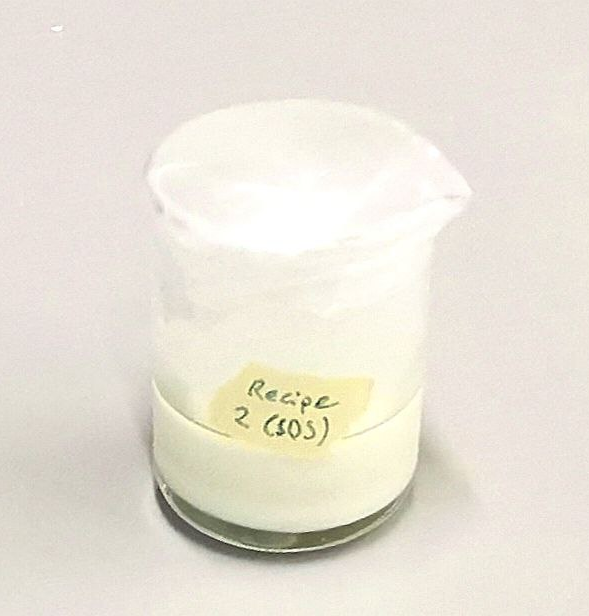
\includegraphics[height=0.8\textwidth]{Pics/sol-aq.png}
		\label{fig:sol-aq}
		\caption{Aquatic solution}
	\end{subfigure}
	\begin{subfigure}{0.49\textwidth}
		\centering
		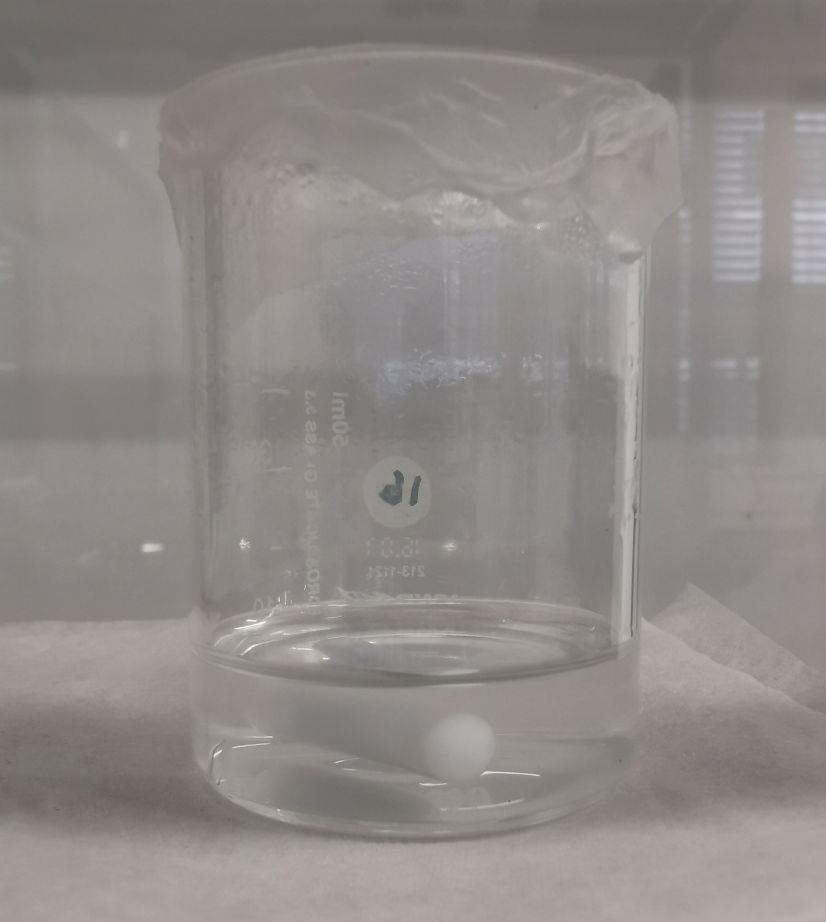
\includegraphics[height=0.8\textwidth]{Pics/sol-bu.png}
		\label{fig:sol-bu}
		\caption{Buthanolic solution}
	\end{subfigure}
	\label{fig:sol}
	\caption{Aquatic and buthanolic solution with magnetic stirring bars in beaker glass sealed with Parafilm} 
\end{figure}

%%%%%%%%%%%%%%%%%%%%%%%%%%%%%%%%%%%%%%%%%%%%%%%%%%%%%%%%%%%%%%%%%%%%%%%%%%%%%%%%%%%%%%%%
%%%%%%%%%%%%%%%%%%%%%%%%%%%%%%%%%%%%%%%%%%%%%%%%%%%%%%%%%%%%%%%%%%%%%%%%%%%%%%%%%%%%%%%%
\subsection{Aquatic solution}\label{sec:exp-sol-aq}
\gls{zrpro} was added to \gls{acac} while stirring and in a separate vessel \gls{water} 
(including any optional additives such as \gls{sds}, \gls{hcl}, \gls{h2so4} or \gls{naoh}) 
was added to \gls{ipo} and both were stirred for one hour. 
These additives were added to influence pH and surface tension with the goal to influence the resulting layer. % \td{see Parvulescu2015}
The \gls{water}-\gls{ipo} mixture was added to the other solution and stirred over night. 
The exact volumes can be taken from table~\ref{tab:rec1}.
Unfortunately, this solution failed to produce anything near homogeneous layers. 
Thus, an alternative solution was found.
%\td{At this point in time everything was doctor bladed by hand. The hight was varied (with tape).}
\begin{table}[h]
	\centering
	\caption{Compositions of different aquatic solutions}
	\label{tab:rec1}
	\begin{tabular}{llllllll}
		\hline
		recipe				&1		&2		&3		&4		&5		&6		&7\\
		\hline
		\gls{zrpro} [\ml{}]	&8		&8		&8		&8		&8		&8		&8\\
		\gls{acac}  [\ml{}]	&8		&8		&8		&8		&8		&8		&8\\
		\gls{ipo}   [\ml{}]	&2		&2		&2		&2		&2		&2		&2\\
		\gls{water} [\ml{}]	&2.6	&2.6	&2.5	&2~		&2		&2		&2\\
		\gls{sds}   [\mg{}]	&-		&5.9	&-		&-		&-		&-		&-\\
		\gls{hcl}   [\ml{}]	&-		&-		&-		&-		&0.5	&-		&-\\
		\gls{h2so4} [\ml{}]	&-		&-		&-		&-		&-		&0.5	&-\\
		\gls{naoh}  [\ml{}] &-		&-		&-		&-		&-		&-		&0.5\\
		\hline
	\end{tabular}
\end{table}
%
%%%%%%%%%%%%%%%%%%%%%%%%%%%%%%%%%%%%%%%%%%%%%%%%%%%%%%%%%%%%%%%%%%%%%%%%%%%%%%%%%%%%%%%%
%%%%%%%%%%%%%%%%%%%%%%%%%%%%%%%%%%%%%%%%%%%%%%%%%%%%%%%%%%%%%%%%%%%%%%%%%%%%%%%%%%%%%%%%
\subsection{Buthanolic solution}\label{sec:exp-sol-bu}
Five different concentrations of the buthanolic solutions were prepared. 
The \gls{1f} was closest to the recipe proposed by Hu et. al. \cite{Hu2016}. 
The other four solutions (\gls{2f}, \gls{3f}, \gls{4f} and \gls{5f}) were similar with 
higher concentrations of \gls{zrpro} (see table \ref{tab:rec2})
with the aim of producing thicker layers.
Not all chemicals mentioned in \cite{Hu2016} were available, so chemically similar 
starting materials had to be chosen from the available inventory. 
%\td{p34}
Different solvents (Butane-1,2-diol, \gls{buoh} and Propan-1-ol) and chelating agents 
(\gls{acac} and citric acid) were tested and later in the process - just before the 
\gls{pso} started - the stabilisation compound (\gls{acoh}) was changed to \gls{ipo}.
The most promising combination of solvent, chelating agent and stabilisation reagent was 
\gls{buoh}, \gls{acac} and \gls{ipo}, respectively, which was used for the final optimisation.
The main differences between the used recipe and the recipe mentioned by \cite{Hu2016} were 
precursor (transition metal complex \gls{zrpro}	\gls{vs} post-transition metal 
complex aluminium isopropoxide), solvent (\gls{buoh} \gls{vs} 2-ethoxyethanol), reaction temperature 
(room temperature \gls{vs} \SI{105}{\celsius}), stirring time (15/15/\SI{30}{\minute}
\gls{vs} 30/30/\SI{120}{\minute}), application process (doctor blading \gls{vs} spin coating), 
the heat treatment between layers (\SI{200}{\celsius} \gls{vs} \SI{200}{\celsius} and then \SI{400}
{\celsius}) and the calcination temperature (\SI{400}{\celsius} \gls{vs}
\SI{500}{\celsius}).
%me          hu
%Zr(OPr)4    Al(iPrO)3   
%1-BuOH      2-MeO-EtOH  
%RT          80-105
%15-15-30    30-30-120
%DB          spin coating
%200C        200/400C
%400C        500C
%%%%%%%%%%%%%%%%%%%%%%%%%%%%%%%%%%%%%%%%

\begin{table}[h]
	\centering
	\caption{Composition of different buthanolic solutions}
	\label{tab:rec2}
	\begin{tabular}{rlllll}
		\hline
		recipe	&1F		&2F		&3F		&4F		&5F		\\
		\hline
		\gls{buoh} [\ml{}]		&4.95	&4.9	&4.85	&4.8	&4.75	\\
		\gls{zrpro} [\ml{}]	&0.05	&0.1	&0.15	&0.2	&0.25	\\
		\gls{acac} [\ml{}]		&0.0125	&0.025	&0.0375	&0.05	&0.0625	\\
		\gls{ipo}/\gls{acoh} [\ml{}]		&2		&2		&2		&2		&2		\\
		\hline
	\end{tabular}
\end{table}

The solvent (\gls{buoh}) was put into a beaker glass (or similar, preferably with an 
air-tight cap) with a magnetic stirring bar and \gls{zrpro} was added while stirring. After 
stirring \minutes{\ds{10 to }15} one mole equivalent chelating agent (\gls{acac}) was 
added and stirred for another \minutes{\ds{10 to }15}. Finally, the stabilisation 
solvent\cite{Hu2016} (\gls{ipo} or \gls{acoh}) was added to the mixture and stirred for 
additional \minutes{\ds{20-}30}. 
In order to make a \gls{2f} solution, the volume of \gls{zrpro} and \gls{acac} was 
doubled and the volume of \gls{buoh} was decreased by the increase of volume of \gls{zrpro}. 

%%%%%%%%%%%%%%%%%%%%%%%%%%%%%%%%%%%%%%%%%%%%%%%%%%%%%%%%%%%%%%%%%%%%%%%%%%%%%%%%%%%%%%%%
%%%%%%%%%%%%%%%%%%%%%%%%%%%%%%%%%%%%%%%%%%%%%%%%%%%%%%%%%%%%%%%%%%%%%%%%%%%%%%%%%%%%%%%%
\section{Doctor blading}
\label{sec:exp-db}
All glass substrates were doctor bladed manually with a smooth stainless steel wire bar 
coater. On two opposing edges adhesive tape was applied to create a valley in between. After the 
layer was applied and dried the tape was removed and the substrate treated with heat.
Lower \gls{db} velocities resulted in less homogeneous layers.
Thus, the \gls{db} wasn't altered in the manual \gls{db} process. 
One and two layers of adhesive tape were used to alter the depth of the valley. 

%Most steel substrates (all pre-optimisation and optimisation samples) 
All steel substrates 
were doctor bladed with 
an Erichsen Coatmaster 510 film applicator with a heatable plate.
The rest was doctor bladed on a glass plate, initially fixed with double sided adhesive tape and 
partially heated with a heat gun.
The blade height was varied from \SI{0}{\milli\meter} to \SI{0.35}{\milli\meter} in 
\SI{0.05}{\milli\meter} steps and did not substantially alter the results.
For the rest of the experiments a blade height of \SI{0.2}{\milli\meter} was used.
%
Eventually, a heatable vacuum plate was used. It 
had equally spaced circular \SI{2.5}{\milli\meter} diameter patches of porous metal where 
underpressure could be applied to keep the substrate in place (see 
figure~\ref{fig:eric}). 
Most of them were covered with tape to increase the suction at the remaining ones. 
After setting the temperature of the heating plate to 
\SI{200}{\celsius}, the vacuum plate temperature (room temperature, \SI{40}{\celsius}, 
\SI{50}{\celsius}, \SI{60}{\celsius}, \SI{70}{\celsius} or \SI{80}{\celsius}) and the 
\gls{db} velocity (\mmps{10}, \mmps{12}, \mmps{14}, \mmps{16}, \mmps{18} or \mmps{20}), 
the blade was put into its original position, the sample was placed on the vacuum plate and the vacuum 
was switched on. 
During pre-optimisation samples, lower \gls{db} velocities (\mmps{0.1}, \mmps{0.5}, 
\mmps{1}, \mmps{2} and \mmps{5}) were tested. 
\ul{100} of solution were 
applied with a 10 - \ul{1000} pipette and the blade moved over the sample distributing the 
liquid evenly. After evaporation of the solution, the vacuum was turned off, the 'blade 
pusher' was put into initial position, the blade was removed and excess solution 
was removed from the plate with a wipe. 
The doctor bladed substrate was transferred to the \SI{200}{\celsius} heating plate and 
rested on there for \minutes{5}. 
This process of applying a \gls{zro} layer was repeated as many times as needed.
\begin{figure}
	\centering
	\begin{subfigure}{.49\textwidth}
		\centering
		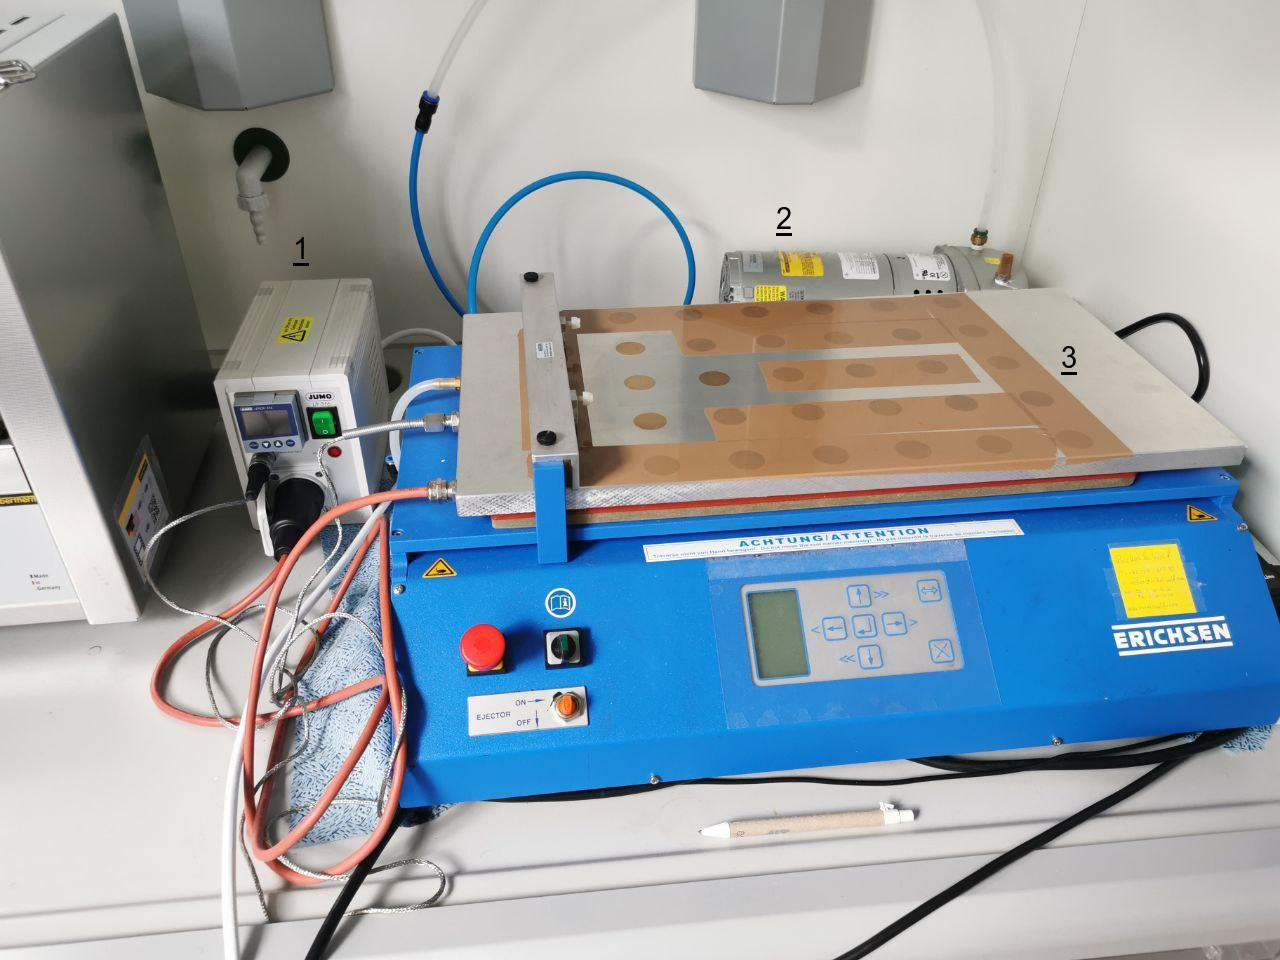
\includegraphics[width=.99\textwidth]{Pics/erichsen1.png}
		\caption{}
	\end{subfigure}
	\begin{subfigure}{.49\textwidth}
		\centering
		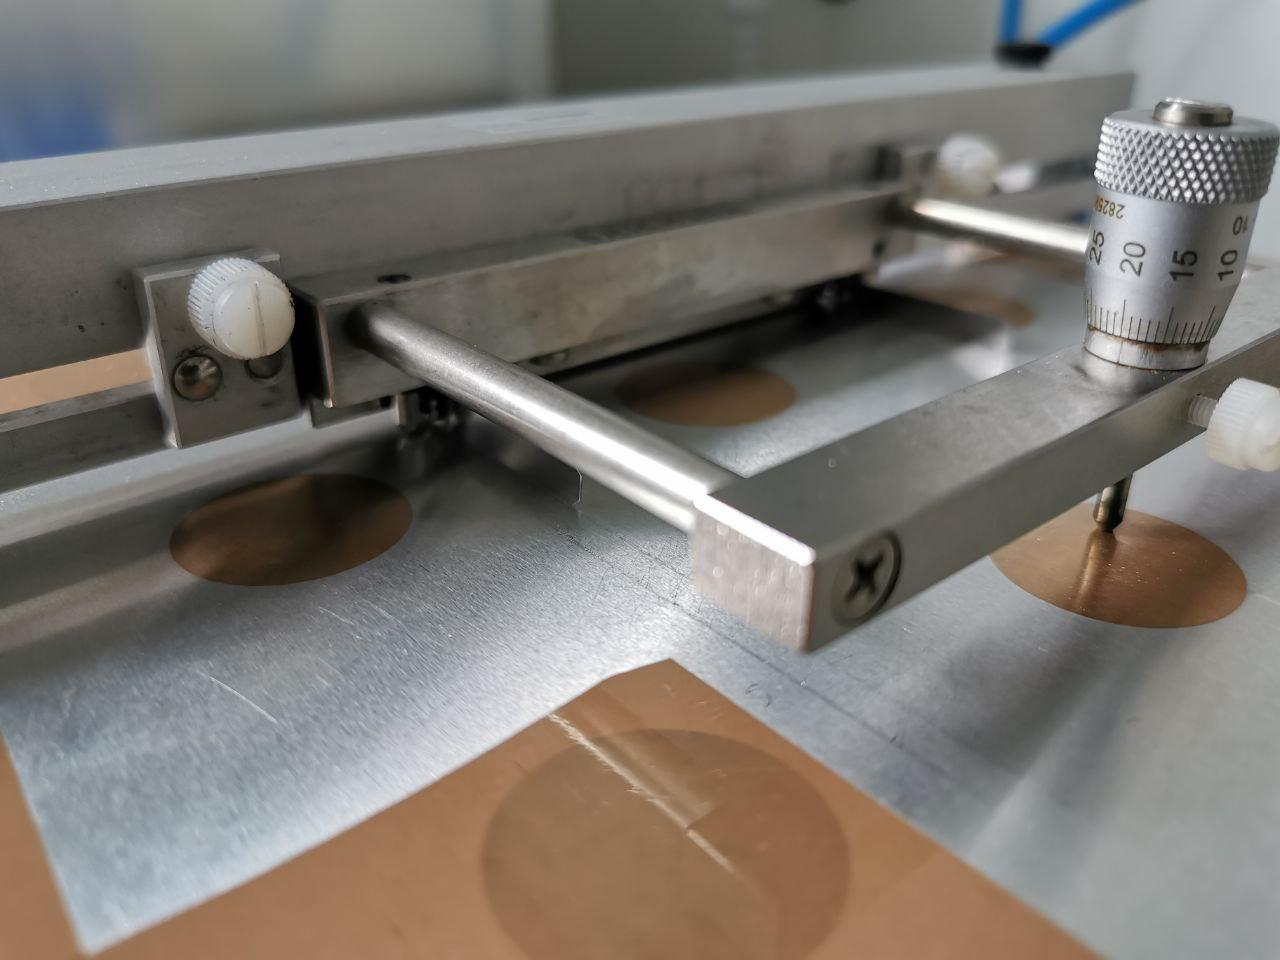
\includegraphics[width=.99\textwidth]{Pics/erichsendb1.png}
		\caption{}
	\end{subfigure}
	\caption{
		(a)
		Temperature regulator (1) on the left,
		vacuum pump (2) in the background and 
		Erichsen Coatmaster 510 film applicator (3) with heatable vacuum plate.
        (b) Close up of the \gls{db} blade in position with blade height adjusted to \SI{0.2}{\micro\meter}.
		The majority of the suction areas is sealed with tape to increase the underpressure at the remaining ones.
	}
	\label{fig:eric}
\end{figure}


%%%%%%%%%%%%%%%%%%%%%%%%%%%%%%%%%%%%%%%%%%%%%%%%%%%%%%%%%%%%%%%%%%%%%%%%%%%%%%%%%%%%%%%%
%%%%%%%%%%%%%%%%%%%%%%%%%%%%%%%%%%%%%%%%%%%%%%%%%%%%%%%%%%%%%%%%%%%%%%%%%%%%%%%%%%%%%%%%
\section{Calcination}\label{sec:exp-calc}
A LabTech EH45C heating plate and a Naberterm LB410 muffle furnace were used to calcinate 
the doctor bladed samples. 
The heating plate could hold temperature for a certain amount of time, but heated with a 
fixed rate of circa \oc{10}/\minutes{}.
In order to achieve a lower overall heating rate several temperature ramps and plateaus 
were alternated (see table~\ref{tab:labtech}). % and figure~\ref{fig:heat}).
This heating procedure was called HP1.
The HP1 procedure was optimized for the available hardware by a colleague working on the 
project prior to the author.

\begin{table}[h]
	\centering
    \caption{Heating programs}
	\label{tab:heating}
    \subcaption{Heating program HP1 used with the Labtech EH45C heating plate}
	\label{tab:labtech}
	\begin{tabular}{rl ll ll ll ll ll ll }%ll ll ll ll ll ll ll}
		\hline
		\hline
		T [\oc{}]	    &80		&100	&150	&160	&170 	&180	&190	&200	&250	&300	&350	&400	\\
		t [\minutes{}]	&10 	&10		&5 		&5 		&5 		&5 &5 &10 &10 &10 &10 &60 \\
		\hline
		\hline
	\end{tabular}
%%%%%%%%%%%%
    \subcaption{Heating programs NT1 - NT6 used with the Naberterm LB410 muffle furnace}
	\label{tab:nt}
	\begin{tabular}{rl ll ll}% ll ll ll ll }%ll ll ll ll ll ll ll}
		\hline\hline
		Name	&80-150\oc{} [\oc{}/\minutes{}]	&150-200\oc{} [\oc{}/\minutes{}]	&200\oc{}-T$_{\textrm{Cal}}$ [\oc{}/\minutes{}]	&T$_{\textrm{Cal}}$ [\oc{}] &t$_{\textrm{Cal}}$ [\minutes{}]	\\
		\hline
		NT1		&2					&1					&2				&400	&60  \\
		NT2		&2					&2					&2				&400	&60  \\
		NT3		&3					&3					&3				&400	&60  \\
		NT4		&4					&4					&4				&400	&60  \\
		NT5		&4					&4					&4				&500	&60  \\
		NT6		&1					&1					&1				&400	&60  \\
%		NT7		&max				&max				&max			&600	&60  \\
		\hline\hline
	\end{tabular}
\end{table}
%
%\clearpage
The NT1 heating program was used to mimic the HP1 heating procedure from the heating 
plate in the Naberterm muffle furnace. 
NT2 is an simplification of NT1 and programs NT3~-~NT6 are the same as NT2 with altered 
heating rate and 
NT5 additionally used a calcination temperature T$_{\textrm{Cal}}$ of \SI{500}{\celsius}.
NT2-NT6 had 2 variables (heating rate and calcination temperature) in contrast to 
NT1 which had 4 (three different heating rates and calcination temperature). 
All heating programs were held at the calcination temperature for one hour.
%In figure \ref{fig:heat} the different heating curves are depicted. 
%
%\begin{figure}
%	\centering
%	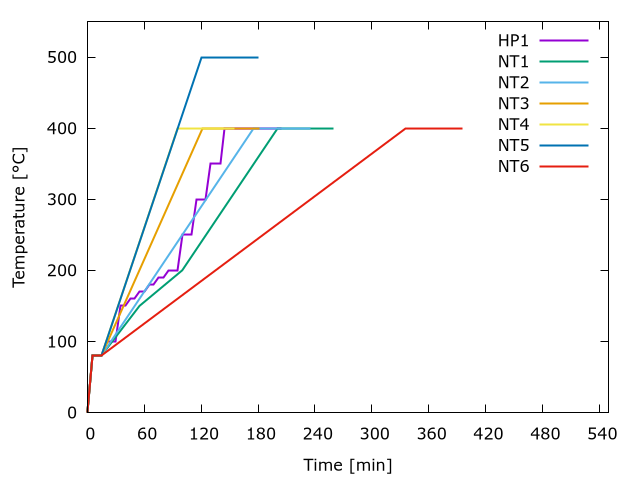
\includegraphics[width=.7\textwidth]{../Data/Graphs/hp1.png}
%	\caption{Different heatings curves}
%	\label{fig:heat}
%\end{figure}

%%%%%%%%%%%%%%%%%%%%%%%%%%%%%%%%%%%%%%%%%%%%%%%%%%%%%%%%%%%%%%%%%%%%%%%%%%%%%%%%%%%%%%%%
%%%%%%%%%%%%%%%%%%%%%%%%%%%%%%%%% CHARACTERISATION %%%%%%%%%%%%%%%%%%%%%%%%%%%%%%%%%%%%%
%%%%%%%%%%%%%%%%%%%%%%%%%%%%%%%%%%%%%%%%%%%%%%%%%%%%%%%%%%%%%%%%%%%%%%%%%%%%%%%%%%%%%%%%
\section{Characterisation}
All \gls{sem} micrographs were taken with a Zeiss Supra 40. 
\Gls{ft}\gls{uv}/\gls{vis}/\gls{nir} transmittance and reflectance spectra (at \SI{20}{\degree} incident 
angle) were recorded with a Bruker Vertex 70 
%transmission [\%] and reflection?  which angle? 
spectrometer with a quartz beam splitter, \SI{0.5}{\milli\meter} aperture and 
Gallium-Phosphide detector for ultra violet light (\SI{303}{\nano\meter} - \SI{588}
% gallium phosphide http://dx.doi.org/10.1051/epjconf/20134800028
{\nano\meter}) and a Silicon detector for visual and \gls{ir} light 
(\SI{500}{\nano\meter} - \SI{1.2}{\micro\meter}). For transmittance the light
entered the sample from the side with the layer. The UV and VIS+IR spectra were merged 
in Opus software. % included in the spectrometer. 
\Gls{xrd} spectra were obtained with a Thermo Scientific ARL Equinox 100 X-Ray Diffractometer. 
All \gls{xrd} spectra were taken at \SI{5}{\degree} incident angle and compared to the internal database.

The \gls{iv} curves were measured with Agilent 4156C Precision Semiconductor 
Parameter Analyzer from \SI{-0.5}{\volt} to \SI{0.5}{\volt} with steps of 
\SI{10}{\milli\volt}.
Prior to \gls{iv} measurements the samples were sputtered with aluminium 
through a mask to produce a multitude of equidistant contacts with a Leybold 
UNIVEX450C Sputter System.
Directional current sputtering was used with Argon as inert gas at \SI{0.005}{\milli\bar} 
and with a power of \SI{40}{\watt} for \SI{700}{\second}.
Between sputtering and \gls{iv} measurements 
direct contacts to the steel substrate were created by removing a patch the \gls{zro}
layer with 
sand paper on two opposing edges of a sample and then by applying silver paste.
See figure~\ref{fig:circuit} for a sketch of the connectivity.

\begin{figure}[hbt]
    \centering
    \begin{circuitikz} \draw
        (0,0) to[european voltage source] (0,2)
        to[ammeter] (2,2) 
        to[generic,l=W] (4,2) 
        to[generic,l=Au] (6,2) 
        to[generic,l=Al] (8,2)
        -- (8,2)
        to[generic,l=ZrO$_2$] (8,0)
        -- (8,0)
        to[generic,l=steel] (6,0)
        to[generic,l=Ag] (4,0)
        to[generic,l=Au] (2,0) 
        to[generic,l=W] (0,0) 
            ;
    \end{circuitikz}
    \caption{Sketch of circuit, from the source clockwise: varibale voltage source, built-in amperometer, gold plated tungsten probe, sputtered aluminium contact, \gls{zro} layer to be measured, steel substrate, dried silver paste contact, gold plated tungsten probe.}
    \label{fig:circuit}
\end{figure}

%%%%%%%%%%%%%%%%%%%%%%%%%%%%%%%%%%%%%%%%%%%%%%%%%%%%%%%%%%%%%%%%%%%%%%%%%%%%%%%%%%%%%%%%
%%%%%%%%%%%%%%%%%%%%%%%%%%%%%%%%%%% PREOPTIMISATION %%%%%%%%%%%%%%%%%%%%%%%%%%%%%%%%%%%%
%%%%%%%%%%%%%%%%%%%%%%%%%%%%%%%%%%%%%%%%%%%%%%%%%%%%%%%%%%%%%%%%%%%%%%%%%%%%%%%%%%%%%%%%
\section{Pre-optimisation}\label{sec:exp-preopt}
%\td{the choice of grenzen for \gls{doe} was done by biotic reinforcement learning (i.e. my brain)}
%\td{Screening}
%The main part of the screening pre-optimisation samples were optimized via biotic reinforcement learning (i.e. my brain). 
The main part of all samples (around 90\%) were pre-optimization samples, 
from which the bulk were screening experiments optimized via biotic reinforcement learning 
(i.e. my brain) in order to obtain reasonable constraints for computerized pre-optimization. 
%Initially, glass plates were doctor bladed manually with aquatic solution and calcinated 
%via HP1. 
%Glass was used because of its availability and in order to be able to make IR 
%\td{transmission} spectra.
%In order to measure the resistivity of the produced layer \gls{fto} and \gls{ito} layered 
%glass plates (both conductive) were used as substrate.
%Conducting substrates were also needed to produce \gls{sem} micrographs. 
%\td{should maybe put this into beginning of section \ref{sec:exp}?}
%otherwise the sample would charge and can't be pictured anymore. 
%this means if the produced layer is thick and homogeneous enough, it's difficult to see in sem
%Different additives were included in the recipe (see table \ref{tab:rec1}) and the resistance was checked with a multimeter. 
%\todo{different additives, heating programs (NT1-NT5 and HP1), blade distances (distance between blade and substrate) and layer counts were tried}
Composition of the aquatic solution, heating program, blade distance (distance between 
blade and substrate) and layer count were varied but no homogeneous layers resulted. 
Thus, 
the buthanolic recipe was introduced, which gave rise to more homogeneous films.
After the blade moved over the substrate the remaining liquid needed about a minute 
to evaporate. 
%\td{
The then current procedure resulted in clear and continuous films, but was plagued from 
inhomogeneities due to drying stains. 
The drying stains could be circumvented by using a heat gun, but the results were not 
reproducible. 
The glass plate of the film applicator was therefore exchanged with a metal plate which 
allowed to hold the sample in place through underpressure and simultaneously heat it to a certain 
temperature. The bounds of the process variables were then explored in a preliminary study 
using the Plackett-Burman\cite{Plackett1946} design implemented in the \texttt{python3} 
library \texttt{pyDOE}. With 
(1,5), (4,10), (400,500), (120,480), (0.1,5) and  (20,80) 
as nominal and extreme values for 
relative concentration of Zr $c_{zr}$, number of layers $\lambda$, calcination temperature $T_{cal}$[\oc{}], heating rate $v_{cal}$[\oc{}/\h{}], \gls{db} velocity $v_{DB}$[\mm{}/\s{}] and \gls{db} temperature $T_{DB}$[\oc{}], respectively. 
After testing the first samples, the lower limit for \gls{db} velocities was altered from 0.1 to 1 (see table \ref{tab:pre-opt1}).
\begin{table}[hbt]
	\centering
	\caption{Pre-optimization experiments}
	\label{tab:pre-opt}
	\begin{subtable}{0.5\linewidth}
		\centering
		\subcaption{Placket-Burman style experiments}
		\label{tab:pre-opt1}
		\begin{tabular}{cccccc}
			\hline
			\hline
	%		&80-150\oc{} [\oc{}/\minutes{}]	&150-200\oc{} [\oc{}/\minutes{}]	&200\oc{}-T$_{\textrm{Cal}}$ [\oc{}/\minutes{}]	&T$_{\textrm{Cal}}$ [\oc{}] &t$_{\textrm{Cal}}$ [\minutes{}]	\\
			$c_{zr}$	&$\lambda$	&$v_{DB}$	&$T_{DB}$	&$v_{cal}$	&$T_{cal}$		\\
			\hline
	1	&10	&5	&20	&120	&400	\\
	1	&4	&0.1	&20	&120	&500	\\
	5	&10	&0.1	&20	&120	&500	\\
	5	&4	&5	&20	&480	&400	\\
	1	&5	&5	&80	&120	&500	\\
	1	&10	&1	&80	&480	&400	\\
	5	&5	&1	&80	&120	&400	\\
	5	&10	&5	&80	&480	&500	\\
			\hline\hline
		\end{tabular}
	\end{subtable}%
	\begin{subtable}{0.5\linewidth}
		\centering
        \subcaption{Hand picked experiments; $^*$varied stabilisation agent}
		\label{tab:pre-opt2}
		\begin{tabular}{cccccc}
	%conc	&layers	&vDOC	&TDOC	&vCal	&Tcal		\\
			\hline\hline
			$c_{zr}$	&$\lambda$	&$v_{DB}$	&$T_{DB}$	&$v_{cal}$	&$T_{cal}$		\\
	%conc	&layers	&$v_{\textrm{DB}}$	&$T_{\textrm{DB}}$	&$v_{\textrm{cal}}$	&$T_{\textrm{cal}}$		\\
			\hline
	2	&8	&0.5	&40	&360	&470	\\
	2	&6	&2	&40	&360	&430	\\
	1	&4	&12	&70	&120	&500	\\
	1	&9	&18	&80	&240	&400	\\
	4$^*$	&6	&14	&60	&240	&500	\\
%	4$^\dagger$	&6	&14	&60	&240	&500	\\
%	4$^\ddagger$	&6	&14	&60	&240	&500	\\
			\hline
			\hline
			\\
%			\multicolumn{6}{c}{*different stabilisation reagent compositions}\\
		\end{tabular}
	\end{subtable}
\end{table}

%$T_{DB}$[\oc{}]
%$v_{DB}$[\mm{}/\s{}]
%$T_{cal}$[\oc{}]
%$v_{cal}$[\oc{}/\h{}]
%Especially the doctor blading velocity.
%}
%It was tried to reduce the waiting time and the resulting \td{drying stains}
%by using a heat gun. The drying was
%accelerated but not reproducibly and the glass plate on the film applicator was changed 
%against the heatable plate.
%With this new buthanolic recipe and heatable plate the limits of the optimization problem 
%were explored in a preliminary study using the Plackett-Burman \cite{Plackett1946} design 
%implemented in the \texttt{python3} library \texttt{pyDOE}.
%For the preliminary study a DB machine and NT were used and the steel. 
\ds{In the preliminary study only steel was used as substrate.}
%The Plackett-Burman \cite{Plackett1946} design implemented in the python3 library \texttt{pyDOE} was used to
%get an overview of reasonable boundaries.
%Latin squares were used to chose which experiments should be ausgefuehrt to get an ueberblick of the optimization room.
%See Code/Input_DOE/make_*exps.py and Code/Input_DOE/mail_theo
Some additional hand picked experiments (see table \ref{tab:pre-opt2}) were introduced to further narrow down the limits of 
the optimization as every reduction in variables or levels meant a faster convergence.
%ooooh 
%%%%%%%%%%%%%%%%%%%%%%%%%%%%%%%%%%%%%%%%%%%%%%%%%%%%%%%%%%%%%%
Shortly before the \gls{pso} the stabilisation agent was changed from \gls{acoh} to 
\gls{ipo} because of much better solution stability.
The - up to this moment - best process was chosen to be tested with 
\ml{1} \gls{acoh}, \ml{0.5} \gls{acoh} plus \ml{0.5} \gls{ipo} and \ml{1} \gls{ipo}.
%\td{As the sample showed the best all ex were proceeded with ipo as stabilisation agent. }
The sample produced with \gls{ipo} as stabilization agent 
showed comparable passivization results and better stability. 
Therefore \gls{ipo} was used  as stabilisation in further experiments.
After the boundaries of the solution were fixed 
the process variables to produce an insulating layer was examined. 
%There were many variables which had to be taken into account. 
%\td{plachett-burman design of experiment with conc, layers, calcination temperature, heating rate, DB velocity and DB temperature as input variables.}
See table \ref{tab:space} for the space spanned for the optimisation.
\begin{table}[ht!]
	\centering
	\caption{Final values used in the \gls{pso}.}
    \label{tab:space}
    \begin{tabular}{cccccc}
        \hline\hline
		$c_{zr}$	&$\lambda$	&$v_{DB}$	&$T_{DB}$	&$v_{cal}$	&$T_{cal}$		\\
%        concentration   &layers &\gls{db} velocity  &\gls{db} temperature   &heating rate   &calcination temperature    \\
        \hline
        2   &4  &10 &40 &120    &300    \\
        3   &6  &12 &50 &360    &400    \\
        4   &8  &14 &60 &600    &500    \\
        5   &10 &16 &70 &840    &       \\
            &12 &18 &80 &1080   &       \\
            &   &20 &   &       &       \\
        \hline\hline
    \end{tabular}
\end{table}

\ds{The final boundaries were
conc 2 - 5 (1) ,
layers 4 - 12 (2),
\gls{db} velocity 10 - 20 (2),
\gls{db} temperature 20 - 80 (20),
heating rate 120 - 1080 (240),
calcination temp 300 - 500 (100),
.
}


\clearpage

%%%%%%%%%%%%%%%%%%%%%%%%%%%%%%%%%%%%%%%%%%%%%%%%%%%%%%%
%%%%%%%%%%%% 5 COMPUTATIONAL DETAILS %%%%%%%%%%%%%%%%%%
%%%%%%%%%%%%%%%%%%%%%%%%%%%%%%%%%%%%%%%%%%%%%%%%%%%%%%%
\section{Computational Details}
\label{sec:comp}
%\subsection{Data Processing}
\label{sec:eval}
Reading list
\begin{itemize}
    %\item https://de.wikipedia.org/wiki/Globaler_F-Test
    %\item https://de.wikipedia.org/wiki/Optimale_Versuchsplanung
    %\item Curse of dimensionality scholar
    %\item linear regression von ungar 
    %\item ridge regression + support vector machine
    %\item correlation vs covariance
    %\item https://en.wikipedia.org/wiki/Regression_analysis
    %\item https://en.wikipedia.org/wiki/Noise_reduction
    %\item https://en.wikipedia.org/wiki/Feature_extraction
    %\item https://en.wikipedia.org/wiki/Feature_selection
    %\item https://en.wikipedia.org/wiki/Dimensionality_reduction
    %\item file:///home/pur/Doc/Uni/Chemie_Master/Int_AIT/Int.git/Code/ML/98_things_can_go_wrong_in_ML_project.html
    %\item https://scikit-learn.org/stable/modules/generated/sklearn.decomposition.PCA.html
    %\item https://scikit-learn.org/stable/modules/generated/sklearn.decomposition.KernelPCA.html#sklearn.decomposition.KernelPCA
    \item 
    \item 
    \item 
\end{itemize}
%\td{describe problem and solution found}
For every sample multiple \gls{iv} curves were measured. 
The main difficulty faced in processing the data was to present the measurements obtain 
from a sample in one representative number. 
The average of each conductance would be an obvious choice but difficult to represent a 
sample correctly since the possible values of conductance span accross several magnitudes.
So the average of logarithms of conductances is the next nearby ansatz.
\todo{why didn't i just take this?}
\td{L2 norm because it might be easier to compare to other methods. }
\td{inspired by euclidean norm/L2 distance from ideal case} 
\td{wanted to put more weight on bad shunts}
\td{plot avg, avg(log), avg(log-13)}

For every I-V curve (aluminium dot) the gradient $g$ at $V=0$ is calculated by taking 
each $n=5$ points after and before the origin at least $d=2$ points distance (which boils
down to the values from \SI{0.02}{\volt} to \SI{0.07}{\volt}) , averaging their V and I values 
and calculating
\begin{equation}
    g = \frac{I_{+m+d} - I_n}{V_{n+1} - V_n}.
\end{equation}
As a measure of conductance a distance D from an ideal non-conducting case. The average of the negative base 10 logarithm subtracted from an ideal non-conducting gradient of $10^{-13}$ 
\begin{equation}
	D = \sum_i^N \frac{ -log_{10}(g_i) - 13}{N}
	\label{eq:D}
\end{equation}
Another measure is the density of shorted species $\rho_{s}$ is calculated in following way:
\begin{equation}
	s_i = \begin{cases}
	1 &\text{if} \quad -log(g_i) < 5 \\
	0 &\text{if} \quad -log(g_i) \geq 5 \\
	\end{cases}
\end{equation}
\begin{equation}
	\rho_s = \sum_i^N \frac{s_i}{N}
	\label{eq:rho}
\end{equation}
Other estimates of the conductance are the averages:
\begin{equation}
	G_1 = log \left( \sum_i^N \frac{g_i}{N} \right)
\end{equation}

\begin{equation}
	G_2 =  \sum_i^N \frac{log(g_i)}{N}
\end{equation}

\subsection{Sample Selection}
\label{sec:ss}
An evolutionary approach was chosen, namely a multi-objective Particle Swarm Optimization (PSO) with a multi-response
Multivariate Adaptive Regression Splines (MARS) model\cite{Villanova2010,Kennedy1995,Breiman1997,Carta2011}.
%
"PSO is a population based heuristic inspired by the flocking behavior of birds. 
To simulate the behavior of a swarm, each bird (or particle) is allowed to fly towards the optimum solution."\cite{Villanova2010}
%
Initially the input parameters (independent variables), their boundaries and number of equidistant levels for each parameter are declared (see table \ref{tab:input}).
Next, the output variables (dependant variables), their weights in the objective function (the function which should be optimized) are specified and if they should be minimized or maximized is noted.
%
%An initial population of particles, i.e. experiments with certain parameters, is chosen out of the population space (space spanned by all possible combinations of input parameters), 
\begin{table}[htb]
	\centering
	\begin{tabular}{cc cc cc}
		\hline
		Zr(PrO)$_4$ conc. [21 g/L]	&layers	&$T_{DB}$[\oc{}]	&$v_{DB}$[\mm{}/\s{}]	&$T_{cal}$[\oc{}]	&$v_{cal}$[\oc{}/\h{}]	\\
		\hline
		2				&4		&40					&10				&300				&120	\\
		3				&6		&50					&12				&400				&360	\\
		4				&8		&60					&14				&500				&600	\\
		5				&10		&70					&16				&					&840	\\
						&12		&80					&18				&					&1080	\\
						&		&					&20				&					&		\\
		\hline
	\end{tabular}
	\caption{Discrete levels of each input parameter \td{are concentrations correct?}}
	\label{tab:input}
\end{table}

The first step is to select an initial population (ensemble of experiments), which is chosen randomly from the population space. 
The samples are made, measured and evaluated according to section \ref{sec:exp} and the distance $D$ (see eq. \ref{eq:D}), $\rho_s$ (see eq. \ref{eq:rho}), $n_{layers}$ (numbers of layers) and $v_{cal}$ (heating rate of calcination process in \oc{}/\minutes{}) are supplied to the program. 
The program uses this data to estimate a response for each output variable (and to choose a fraction of the initial population which is allowed to propagate).
The response variables for the entire population space is calculated. 
The current population - each of the particles independently - moves towards the optimum solution.
The population for the next time step is outputted and the experiments are again executed, measured and evaluated.

%\subsection{EMMA Propagation}
\begin{table}[htb]
	\centering
	\begin{tabular}{ccccccc}
		\hline
		\hline
conc	&layers	&vDOC	&TDOC	&vCal	&Tcal	&	\\
		\hline
1	&10	&5	&20	&120	&400	&\\
1	&4	&0.1	&20	&120	&500	&\\
5	&10	&0.1	&20	&120	&500	&\\
5	&4	&5	&20	&480	&400	&\\
1	&5	&5	&80	&120	&500	&\\
1	&10	&1	&80	&480	&400	&\\
5	&5	&1	&80	&120	&400	&\\
5	&10	&5	&80	&480	&500	&\\
2	&8	&0.5	&40	&360	&470	&\\
2	&6	&2	&40	&360	&430	&\\
		\hline
%4	&12	&-	&-	&-	&-&\\
1	&4	&12	&70	&120	&500	&\\
1	&9	&18	&80	&240	&400	&\\
%2	&5	&18	&70	&-	&-		&\\
4	&6	&14	&60	&240	&500	&\\
4	&6	&14	&60	&240	&500	&\\
4	&6	&14	&60	&240	&500	&\\
		\hline
2	&10	&20	&40	&120	&500	&6113\\
3	&8	&18	&70	&1080	&300	&2850\\
3	&6	&10	&50	&1080	&400	&5526	\\
%3	&10	&14	&50	&600	&500	&-7374	\\
3	&10	&16	&80	&120	&500	&6554	\\
4	&6	&16	&80	&1080	&300	&2947	\\
3	&12	&12	&80	&840	&500	&8318	\\
3	&10	&14	&50	&600	&500	&7374	\\
5	&6	&10	&60	&1080	&400	&5648	\\
5	&10	&20	&60	&360	&300	&3956	\\
5	&12	&14	&60	&1080	&300	&2700	\\
		\hline
%2	&2	&10	&40	&600	&300	&-7201	\\
2	&4	&10	&80	&1080	&300	&6101	\\
%2	&4	&10	&40	&600	&300	&-7201	\\
2	&4	&10	&40	&600	&300	&7201	\\
3	&4	&12	&60	&600	&300	&1462	\\
4	&4	&10	&80	&1080	&300	&2883	\\
5	&12	&20	&70	&600	&300	&1680	\\
		\hline
2	&4	&10	&40	&120	&300	&1	\\
2	&4	&10	&40	&120	&500	&6001	\\
3	&4	&10	&40	&120	&500	&6102	\\
5	&4	&10	&80	&1080	&300	&2884	\\
5	&12	&20	&60	&120	&300	&360	\\
		\hline
3	&4	&10	&40	&600	&400	&4202	\\
2	&6	&20	&40	&120	&500	&6105	\\
%4	&4	&14	&80	&1080	&300	&-2923	\\
5	&12	&14	&60	&600	&300	&1500	\\
3	&6	&14	&60	&600	&300	&1486	\\
4	&4	&14	&80	&1080	&300	&2923	\\
		\hline
4	&8	&18	&80	&1080	&300	&2971	\\
3	&8	&10	&50	&1080	&300	&2530	\\
2	&12	&16	&40	&120	&400	&3077	\\
2	&10	&18	&60	&1080	&300	&2733	\\
4	&10	&10	&50	&1080	&300	&2535	\\
		\hline
		\hline
	\end{tabular}
	\caption{}
	\label{tab:emma}
\end{table}



\subsection{Fitting via Machine Learning}
\td{scarce data may lead to overfitting\cite{Lecun1995conv}}\\
Python and sci-kit learn \td{cite} was used to implement a linear fit model, and SVR with the kernels polynomial, rbf and sigmoid. 
The space of hyper parameters C, the degree (in case of polynomial), epsilon and gamma was scaned. 

The independent variables are located on a partially irregular grid.  


%\clearpage

%%%%%%%%%%%%%%%%%%%%%%%%%%%%%%%%%%%%%%%%%%%%%%%%%%%%%%%
%%%%%%%%%%%%%% 6 RESULTS AND DISCUSSION %%%%%%%%%%%%%%%
%%%%%%%%%%%%%%%%%%%%%%%%%%%%%%%%%%%%%%%%%%%%%%%%%%%%%%%
\section{Results and Discussion}
\label{sec:results}
%%%%%%%%%%%%%%%%%%%%%%%%%%%%%%%%%%%%%%%%%%%%%%%%%%%%%%%%%%%%
and cite something pro forma \cite{ncbi1butanol}
%%%%%%%%%%%%%%%%%%%%%%%%%%%%%%%%%%%%%%%%%%%%%%%%%%%%%%%%%%%
%%%%%%%%%%%%%%%%%%%%%%%%%%%%%%%%%%%%%%%%%%%%%%%%%%%%%%%%%%%
\subsection{Material Scientific}
\subsubsection{Solution}
As already indicated in the experimental section the recipe adopted from \cite{Anwar2017} didn't produce any \td{good} results. 
The solution was milky/cloudy and didn't produce homogeneous films. 
Altering the composition, pH, surfactant etc. didn't improve the resulting \gls{zro} layers. 
%- first recipe tried to improve to achieve more restisting layer. by pH value, surface tension and solution ratios (only 10\% change because it was assumed, that the recipe is good and should be improved, but the recipe should be altered thoroughly. two layers were also tried but didn't even pass the visual examination/test/inspection. A curst was produced. 

The sol-gel recipe optimized by \cite{Hu2016} for \ch{Al2O3} worked splendidly for our use even after (not so) minor changes.
%An substantial improvement could be achieved by
The stability of the solution could be increased a lot by replacing the stabilizing agent (\gls{acoh}) with \gls{ipo}.
The stability was inspected visually. 
As soon as the solution showed initial cloudiness, it was declared as unstable. 
The regular solution was stable for approximately \td{24h} sealed with Parafilm. 
%192 was first with IPOH
A solution with \gls{ipo} as stabilizing agent stayed stable for \td{72h}. 
As an increase of the \gls{zrpro} concentration decreased the \td{stable time}. 
%5F ca 100min
%4F ca 140min
%3F ca 420min (7h)
%extra AcOH stabilzed but needed so much that dilution too large...
%\td{IPO influence on "stability" p74: 600ul IPO makes clear, 4000 ul BuOH not clear with 
%same base solution (1ml of 4F), added extra 400ul to BuOH sol and after 5min clear. 
%of 1:5 is unacceptable Dilution }
%- 21.8 (1F) from 15.02. 13:30 bis 
%26.3 (1ml iPO to ca2ml of 5f) from 16.02. 16:30 bis 18.02.++
%18.02 4F in 80min milky
%      2F in ca 24h (stabilization AcOH)
%
%acceptable layer was produced by buthanolic solution, but very unstable (short lived) how long? p41 
\Gls{ipo} solution allowed to even reuse high concentrated solution, which would otherwise become cloudy under 60 minutes. 
Multiple question still need to be answered: 
What causes the cloudiness (as stability increased through sealing probably \ch{H2O} from the air or \ch{O2}) and what's the mechanism? 
How does \gls{ipo} increase the stability? 
Does it do so because it "fits" better with the solvent. 
As the original solvent was 2-methoxy-ethonanol instead of \ch{buoh}. 
It was even observed that the addition of \td{some drops of} \gls{ipo} to an acetic solution can clear the solution.
5F acetic solution milky over night 5:1 dilution with \gls{ipo} and clear after one minute of stirring and stayed clear over 5 nights.
% more details on pages 68ff
No effect on the solution or the resulting layer was noticed \td{from the initial stirring}
\todo{Following stirring times (in minutes) were tested and didn't have an influence on stability of the solution: 10-10-20, 10-10-45, 30-30-180.}
%The stirring time was untersucht, but not much difference so shortest was used because 
%short time can produces faster and the resulting solution is longer stable 
%(after finishing mixing)

%\td{instead of changing the stabilisation agent before optimisation, could change after pso, was vor und nachteile?}
after realizing the improved effectiveness of \gls{ipo} for experimentation, 
it was decided that EMMA will be executed with \gls{ipo} solution.
\begin{figure}
    \centering
    \begin{subfigure}{.3\textwidth}
        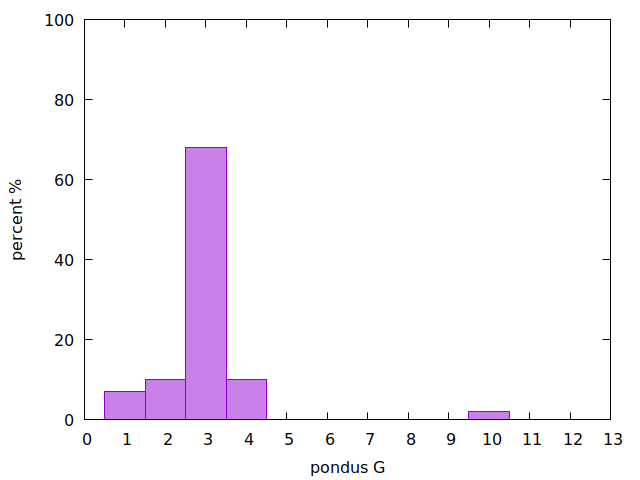
\includegraphics[width=\textwidth]{Pics/iv/iv-199-acoh.png}
        \caption{iv acoh} \label{fig:iv-acoh}
    \end{subfigure}
    \begin{subfigure}{.3\textwidth}
        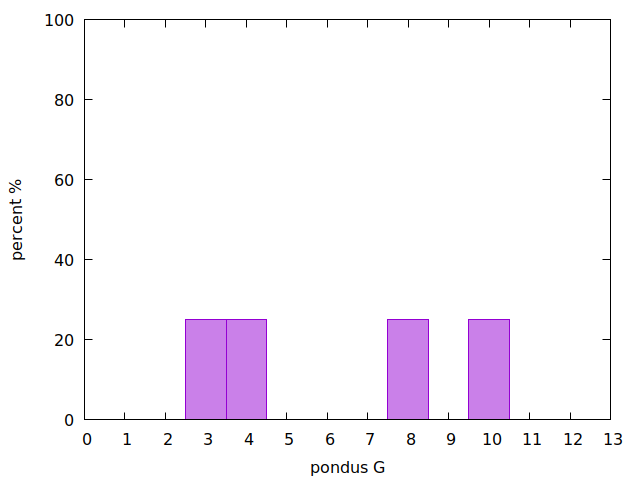
\includegraphics[width=\textwidth]{Pics/iv/iv-201-acoh-ipo.png}
        \caption{iv acoh ipo} \label{fig:iv-acoh-ipo}
    \end{subfigure}
    \begin{subfigure}{.3\textwidth}
        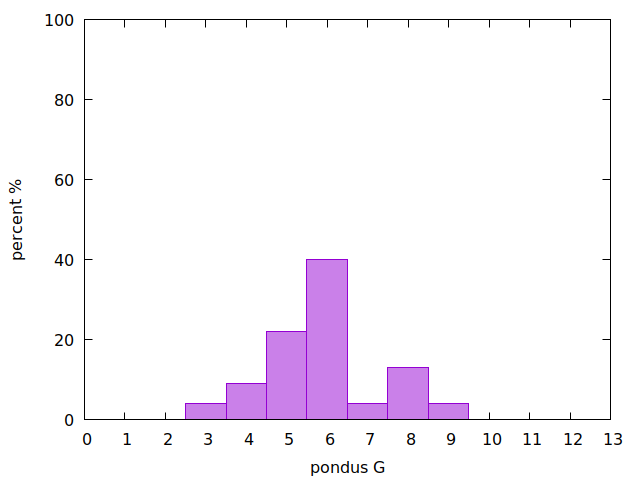
\includegraphics[width=\textwidth]{Pics/iv/iv-192-ipo.png}
        \caption{ipo} \label{fig:ipo}
    \end{subfigure}
    \caption{iv of 6x4F} \label{fig:iv-ipo}
\end{figure}

%\iffalse
%%%%%%%%%%%%%%%%%%%%%%%%%%%%%%%%%%%%%%%%%%%%%%%%%%%%%%%%%%%
%%%%%%%%%%%%%%%%%%%%%%%%%%%%%%%%%%%%%%%%%%%%%%%%%%%%%%%%%%%
\subsubsection{Infra Red}

\begin{figure}
    \centering
    \begin{subfigure}{.49\textwidth}
        \centering
        \includegraphics[width=.99\textwidth]{Pics/ir-gt.png}
        \caption{Transmittance of \gls{zro} on glass} \label{fig:ir-gt}
    \end{subfigure}
    \begin{subfigure}{.49\textwidth}
        \centering
        \includegraphics[width=.99\textwidth]{Pics/ir-gr.png}
        \caption{reflectance of \gls{zro} on glass} \label{fig:ir-gr}
    \end{subfigure}
    \caption{IR} \label{fig:ir}
\end{figure}

In figure \ref{fig:ir-gt} transmission spectra of visible and \gls{nir} light can be seen. 
Each sample had different numbers of layers. 
The incident angle was 0 degree for each sample.
differnt numbers of layers of \gls{zro} on a glass slide with 0 degree incident angle. 
The more layers the more of the light is absorbed (800nm) by the \gls{zro} layers. 
%The trend is not monotonic due to inhomogenities in the sample???b
The thicker the layer is the more wavy the graph, which can be most likely be attributed to interferrence. 
This trend can also be observed in figure \ref{fig:ir-gr}
Figure \ref{fig:ir-gr} shows reflectance spectra of visible and \gls{nir} at an angle of 45 degrees. 
%\fi


%%%%%%%%%%%%%%%%%%%%%%%%%%%%%%%%%%%%%%%%%%%%%%%%%%%%%%%%%%%
%%%%%%%%%%%%%%%%%%%%%%%%%%%%%%%%%%%%%%%%%%%%%%%%%%%%%%%%%%%
\subsubsection{SEM}
\begin{figure}
    \centering
    \begin{subfigure}{.45\textwidth}
        \centering
        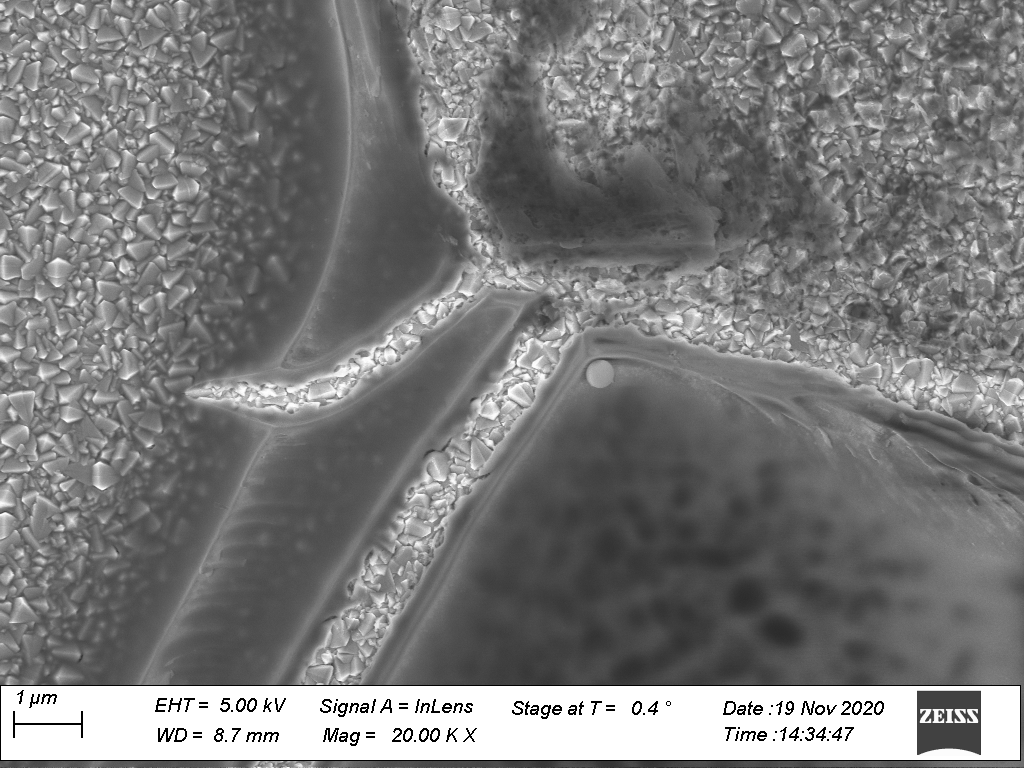
\includegraphics[width=.8\textwidth]{Pics/sem/071_fto_old_1x.png}
        \caption{71 fto old 1x} \label{fig:sem-old1}
    \end{subfigure}
    \begin{subfigure}{.45\textwidth}
        \centering
        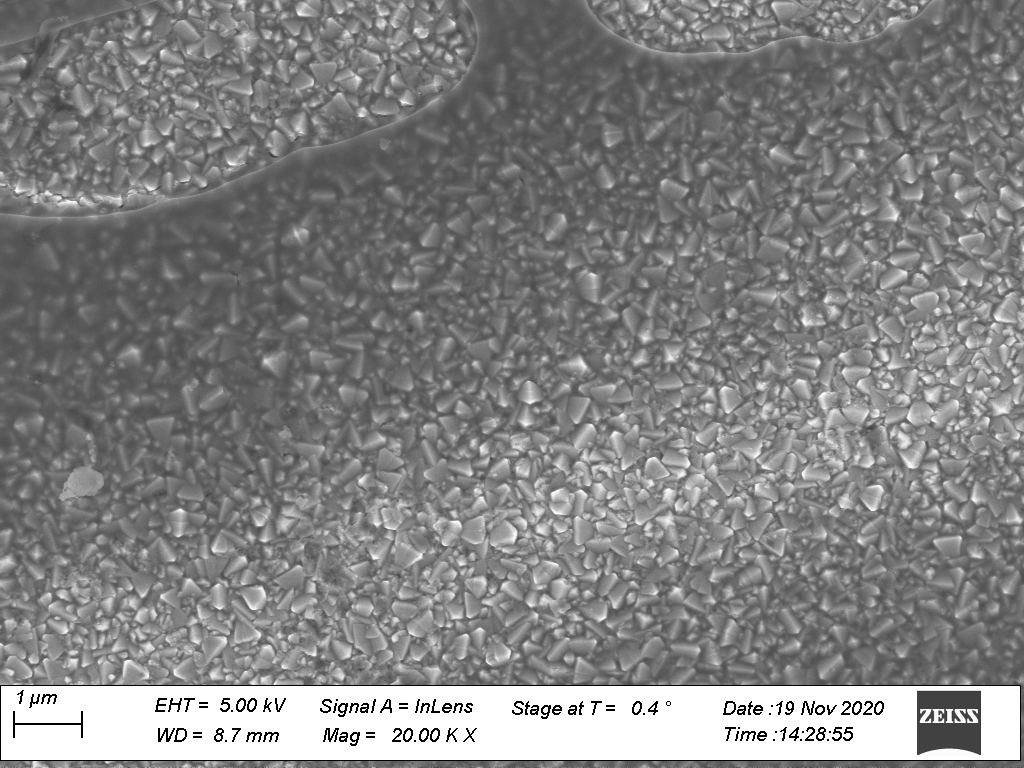
\includegraphics[width=.8\textwidth]{Pics/sem/071_fto_old_2x.png}
        \caption{71 fto old 2x} \label{fig:sem-old2}
    \end{subfigure}
    \begin{subfigure}{.45\textwidth}
        \centering
        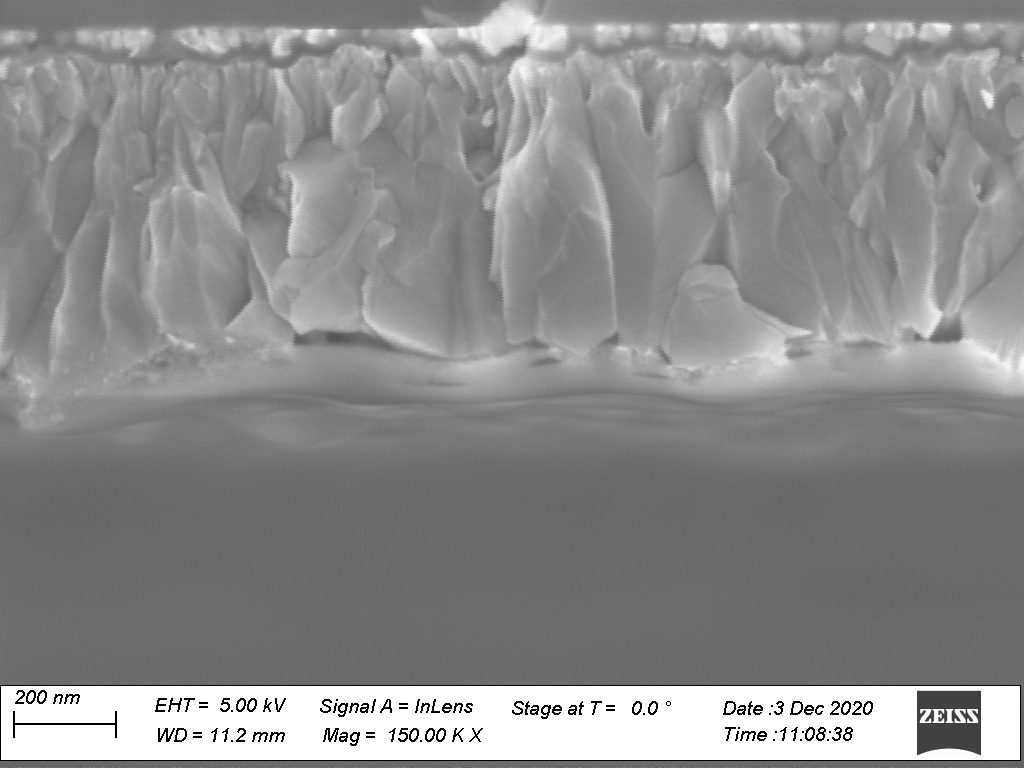
\includegraphics[width=.8\textwidth]{Pics/sem/115_fto_cs_1x.png}
        \caption{115 fto cs 1x} \label{fig:sem-cs1}
    \end{subfigure}
    \begin{subfigure}{.45\textwidth}
        \centering
        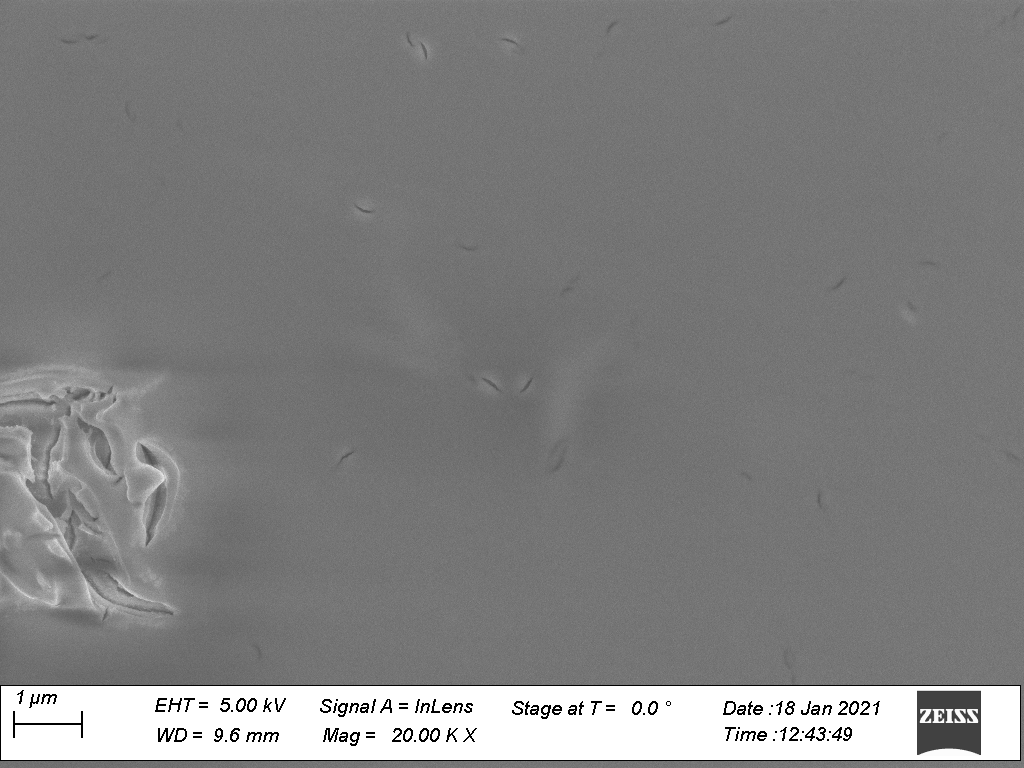
\includegraphics[width=.8\textwidth]{Pics/sem/147_steel_ph_10x.png}
        \caption{147 steel ph? 10x} \label{fig:sem-ph}
    \end{subfigure}
    \caption{sem}
    \label{fig:sem}
\end{figure}

The \gls{sem} pictures were not easy to take since we were trying to create an insulator 
and the quality of the picture relies on the conductance of the material's surface. 
This means that the better the quality of the resulting layer the more tedious it was to get/take a decent SEM image. 
Figures \ref{fig:sem-old1} and \ref{fig:sem-old2} shows ausschnitte of \gls{zro} (dark) on top of \gls{fto} (finely polycrystalline). 
These were the results of a single (figure \ref{fig:sem-old1}) and double (figure \ref{fig:sem-old2}) "layer" of the aquatic recipe. 
Large cracks and inhomogenity were part of (ausmachen) all samples created with the Anwar recipe; 
also/even after several/multiple/various alteration to the recipe. 

Figure \ref{fig:sem-cs1} shows the cross section of a single layers of \gls{zro} on \gls{fto} glass. 
The large crystalline \td{range} which makes up most of the topper/top part of the image is \gls{fto}. 
The úbergang to glass is gerade noch so zu sehen. 
On the lower kante of the \gls{fto} a circa 100nm thick homogeneous layer can be observed, \gls{zro} produced by buthanolic recipe inspired by Hu et al..

Figure \ref{fig:sem-ph} shows a top view of 10 layers of the buthanolic layer on top of a steel substrate. 
The large unregularity on the bottom left could darstellen a pin hole a (tiny) hole that reaches the substrate. 
These unregularites are rather the ausnahme. 
Alternatively, the small, hardly visible  irregularities verstreut across surface could darstellen such pin holes. 
These - I think - eher only are one layer deep irregularities since they are so haeufig 
and very little pin holes were observed on similar samples. 




%%%%%%%%%%%%%%%%%%%%%%%%%%%%%%%%%%%%%%%%%%%%%%%%%%%%%%%%%%%
%%%%%%%%%%%%%%%%%%%%%%%%%%%%%%%%%%%%%%%%%%%%%%%%%%%%%%%%%%%
\subsubsection{Current Voltage Curves} 
\begin{figure}
    \centering
    \begin{subfigure}{.3\textwidth}
        \includegraphics[width=\textwidth]{Pics/iv/log-154-good-3x4F.png}
        \caption{log good 3x4F} \label{fig:iv-log-good}
    \end{subfigure}
    \begin{subfigure}{.3\textwidth}
        \includegraphics[width=\textwidth]{Pics/iv/log-146-okay-10x1F.png}
        \caption{log okay 10x1F} \label{fig:iv-log-okay}
    \end{subfigure}
    \begin{subfigure}{.3\textwidth}
        \includegraphics[width=\textwidth]{Pics/iv/log-156-bad-3x3F.png}
        \caption{log bad 3x3F} \label{fig:iv-log-bad}
    \end{subfigure}
    \begin{subfigure}{.3\textwidth}
        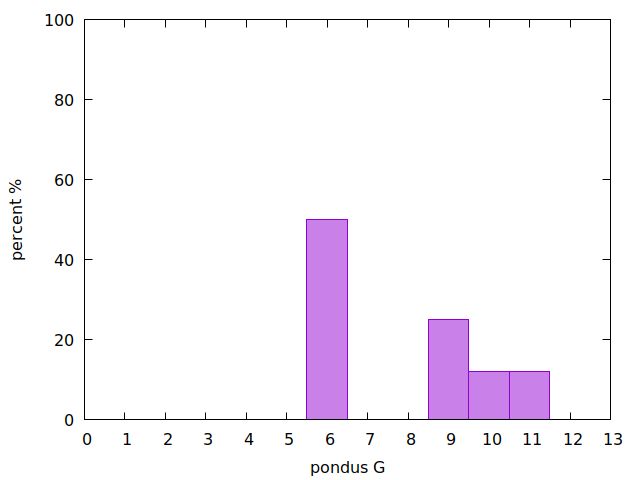
\includegraphics[width=\textwidth]{Pics/iv/stat-154-okay-3x4F.png}
        \caption{stat good 3x4F} \label{fig:iv-stat-good}
    \end{subfigure}
    \begin{subfigure}{.3\textwidth}
        \includegraphics[width=\textwidth]{Pics/iv/stat-146-good-10x1F.png}
        \caption{stat okay 10x1F} \label{fig:iv-stat-okay}
    \end{subfigure}
    \begin{subfigure}{.3\textwidth}
        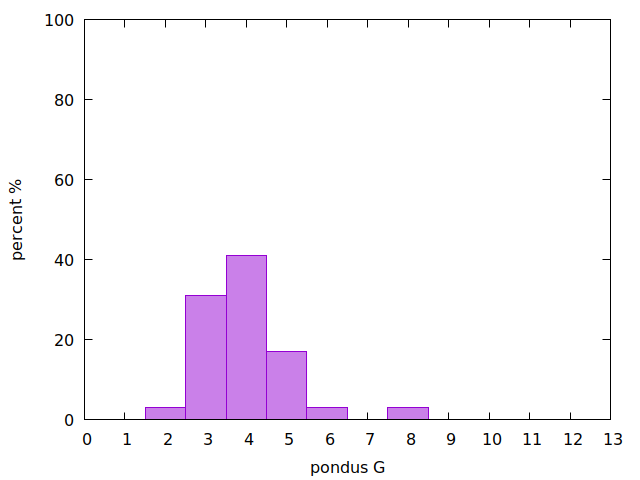
\includegraphics[width=\textwidth]{Pics/iv/stat-156-bad-3x3F.png}
        \caption{stat bad 3x3F} \label{fig:iv-stat-bad}
    \end{subfigure}
    \caption{maybe remove 146 and make 154 good AND set yrange [E-1:E-14] and show phd threshold} \label{fig:iv}
\end{figure}

%Figures \ref{fig:iv-log-good} and \ref{fig:iv-stat-good} are measurements from a good sample. 
Figure \ref{fig:iv-log-good} shows \gls{iv} curves in logarithmic scale of a good sample. 
Each line represents a I-V measurement at a distinct contact 
The highest voltages are around 
All of the curves show a max voltage of under \num{e-6} \SI{}{\volt}. 
And quite a few show hardly any current which is the ideal. 
For each measurement the conductivity (i.e. the gradient at V=0) was calculated (see section \ref{sec:eval}). 
Figure \ref{fig:iv-stat-good} shows the distribution of gradients. 

Figures \ref{fig:iv-log-okay} and \ref{fig:iv-stat-okay} show measurements from moderate sample. 
Most of the \gls{iv}s have a maximum voltage of under \num{e-6} V, but there are some so called pin holes. 

Finally, figures \ref{fig:iv-log-bad} and \ref{fig:iv-stat-bad} show a sample where all 
measurement exhibit relatively high voltages. Which indicates a bad overall \gls{zro} layer. 

%%%%%%%%%%%%%%%%%%%%%%%%%%%%%%%%%%%%%%%%%%%%%%%%%%%%%%%%%%%
%%%%%%%%%%%%%%%%%%%%%%%%%%%%%%%%%%%%%%%%%%%%%%%%%%%%%%%%%%%
\subsubsection{XRD}
\begin{figure}
	\centering
	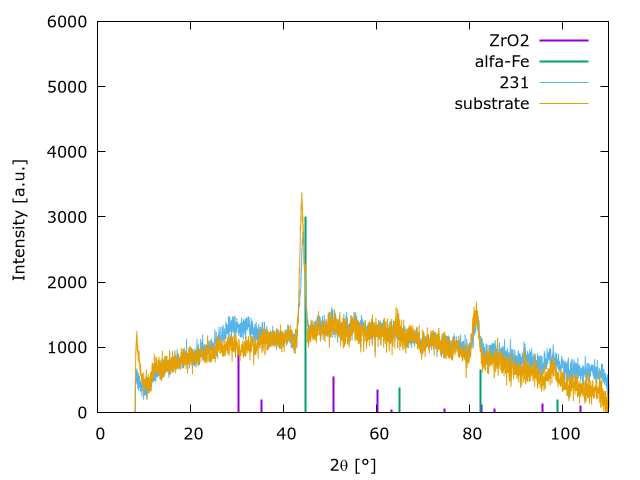
\includegraphics[width=\picwidth]{Pics/xrd.png}
	\caption{XRD spectra}
	\label{fig:xrd}
\end{figure}

In figure \ref{fig:xrd} the two strongest $\alpha$-Fe peaks can be seen clearly. 
The highest peak of \gls{zro} is very \td{broadened} and is therefore not as distinct. 
This wideness is is due to polycristalinity/amorphness of the material which is \td{erwartet due} to the sol-gel creation process. 

%%%%%%%%%%%%%%%%%%%%%%%%%%%%%%%%%%%%%%%%%%%%%%%%%%%%%%%%%%%
%%%%%%%%%%%%%%%%%%%%%%%%%%%%%%%%%%%%%%%%%%%%%%%%%%%%%%%%%%%
\subsubsection{Preoptimization}
The doctor blading velocity (i.e. the velocity with which the blade moves and spreads the sol over the sample) 
was varied during preoptimization. 
The slower the \gls{db} velocity the more \td{homogeneously} the solution evaporated. 
If the \gls{db} was \td{too slow (lt 1 mm/s)} the surface tension pulled solvent over the sample without \td{leaving was zurk/forming a gel.}
\td{deposition because miniscus is pulling liquid off the substrate.}
Additionally the temperature while doctor blading affects the resulting layer together with the \gls{db} velocity. 

\td{Assumption: Ideally solution evaporate shortly after DB but not before}
due to the boiling point of \gls{buoh} at 117 C\cite{ncbi1butanol} the room temperature to 80 C were used as temperature during \gls{db}.
- p76, 146 (10x1F) good, 154 (3x4F) okay, 156 (3x3F) bad visualisation


%%%%%%%%%%%%%%%%%%%%%%%%%%%%%%%%%%%%%%%%%%%%%%%%%%%%%%%%%%%%
%%%%%%%%%%%%%%%%%%%%%%%%%%%%%%%%%%%%%%%%%%%%%%%%%%%%%%%%%%%
\subsection{EMMA}
\label{sec:res-emma}
%%%%%%%%%%%%%%%%%%%%%%%%%%%%%%%%%%%%%%%%%%%%%%%%%%%%%%%%%%%%%%%%%%%%%%%%%%%%%%%%%%%%%%%%5
%%% ALL SAMPLES
A total of 30 recipes (see appendix \ref{sec:app-emma}) have been investigated in 
five iterations ($t = 0, \dots, 4$) of the algorithm. 
Where the first generation encompassed 10 particles and each subsequent generation encompassed 5 particles. 
The best recipes for each generation can be seen in table \ref{tab:emma-Gb}. 
The experiments for generation 5 where not executed but 
predictions were already made
with the information from the previous generations. 
%%% BEST
The best sample predicted by the algorithm is experiment number 13 with 
%lowest solution concentration, second highest layer count, lowest \gls{db} velocity and temperature, 
%and lowest calcination heating rate and temperature. 
lowest $c_{zr}$, $v_{DB}$, $T_{DB}$, $v_{cal}$, $T_{cal}$ and second highest $\lambda$. 
%lowest solution concentration, second highest layer count, lowest \gls{db} velocity and temperature, 
%and lowest calcination heating rate and temperature. 


\begin{table}[htb]
	\centering
    \caption{Global best per generation}
	\label{tab:emma-Gb}
	\begin{tabular}{cccccccc}
        \hline\hline
        generation  &enr &$c_{zr}$ &$\lambda$ &$v_{DB}$ &$T_{DB}$ &$v_{cal}$ &$T_{cal}$\\
        \hline
     1   &1       &2    &4   &10   &40  &120  &300\\
     2   &5       &2    &6   &10   &40  &120  &300\\
     3   &2947    &4    &6   &16   &80 &1080  &300\\
     4   &2405    &2    &6   &10   &40 &1080  &300\\
     5   &13      &2   &10   &10   &40  &120  &300\\
    \hline\hline
	\end{tabular}
\end{table}

\begin{table}
	\centering
    \caption{Predicted $\hat{\gamma}$} 
    \label{tab:emma-pred-G}
    \begin{tabular}{cccccc}
        \hline\hline
    enr &1st gen \gls{rf}   &2nd gen \gls{rf} &3rd gen \gls{rf}    &4th gen \gls{rf}   &5th gen \gls{rf}\\
        \hline
    1       &1.214185    &       &       &       &38.7962       \\
    5       &       &4.196626       &       &       &25.47335       \\
    2947    &       &       &10.9594    &       &10.9594       \\
    2405    &       &       &       &20.04962   &25.47335       \\
    13      &       &       &       &       &24.87178   \\
        \hline\hline
    \end{tabular}
\end{table}

%%% OVER TIME 
The only clear trend from table \ref{tab:emma-Gb} is the layer count, which rises with the generations. 
The remaining input variables remained more or less the same except for the 3rd generation. 
%
In table \ref{tab:emma-pred-G} it can be seen that the predicted $\hat{\gamma}$ 
(predicted with 5th generation \gls{rf}) lowered with each iteration, 
except for sample 2947, which wasn't predicted but measured. 
This shows that the easiest part of the algorithm - the selection of the optimum 
from predicted values - works as expected. 
% and that the predictions included more lower values over time
%
Contrarily, the predicted $\hat{\gamma}$ for each generation's best 
(predicted by the very generation's \gls{rf}) does increase with each iteration 
(see diagonal in table~\ref{tab:emma-pred-G}). 
This indicates an underestimation of $\gamma$ at the beginning and a correction with time. 
%The reason for is probably a 
The underestimation probably stems from a lucky selection of initial experiments or a skew in the measurements. 

In figure \ref{fig:emma-gen} we can see the two measured main \textit{optimizands}, 
$\gamma$ and $\rho$, of each particle at generations 1 to 4. 
%for each particle included in the optimization. 
%It shows a clear trend which indicates that the optimization worked even though 
Both variables were to be minimized and show a clear trend towards low values, 
indicating that the optimization worked even though 
the prediction functions (see equations (\ref{eq:emma-phd3}) - (\ref{eq:emma-vcal4})) 
and the chosen samples where not exactly as expected. 
Neither were the measurements for these samples, which might be due to the high measuring error of samples and variation of quality due to uncontrolled independent variables like room temperature or humidity. 

\begin{figure}[hb]
    \centering
    \begin{subfigure}{.45\textwidth}
        \centering
        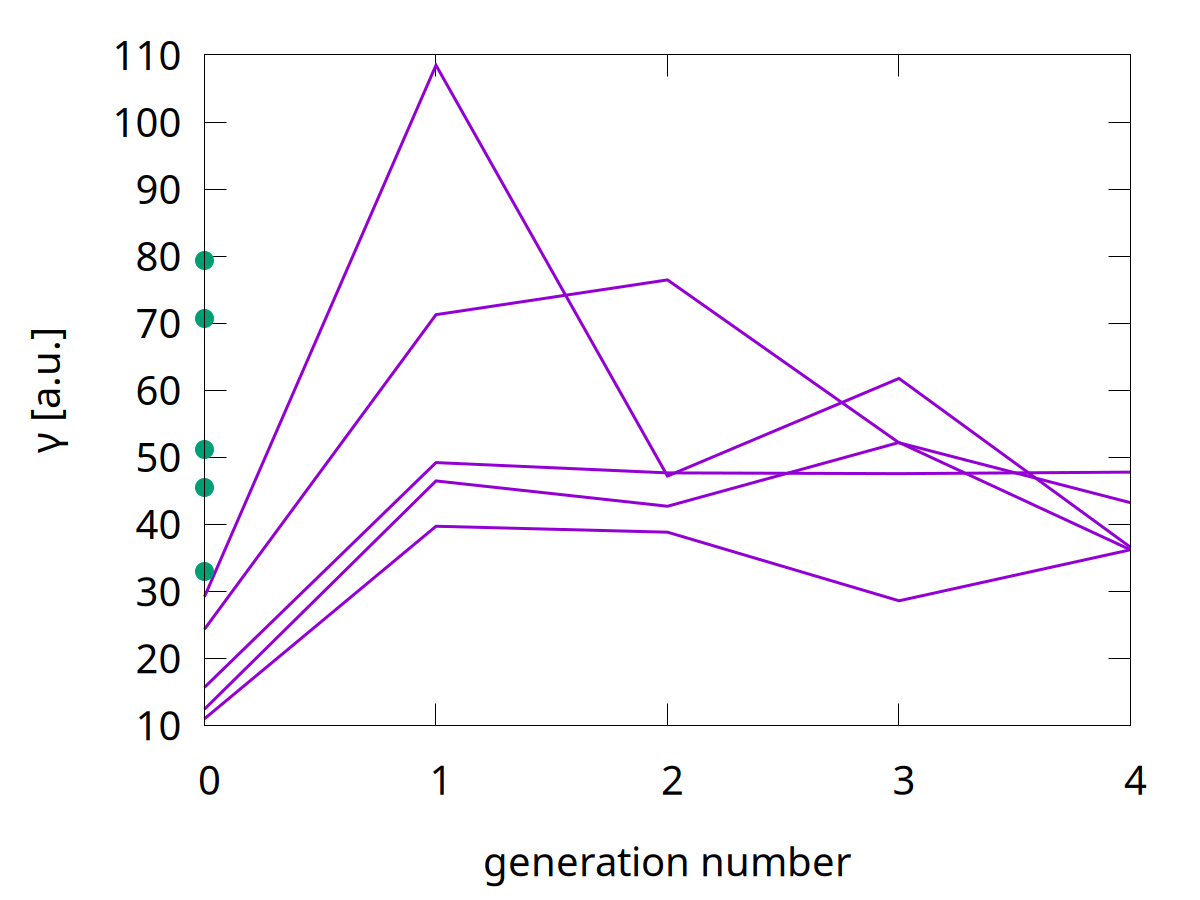
\includegraphics[width=.8\textwidth]{Pics/stats/gen-G.png}
        \caption{} \label{fig:emma-G-gen}
    \end{subfigure}
    \begin{subfigure}{.45\textwidth}
        \centering
        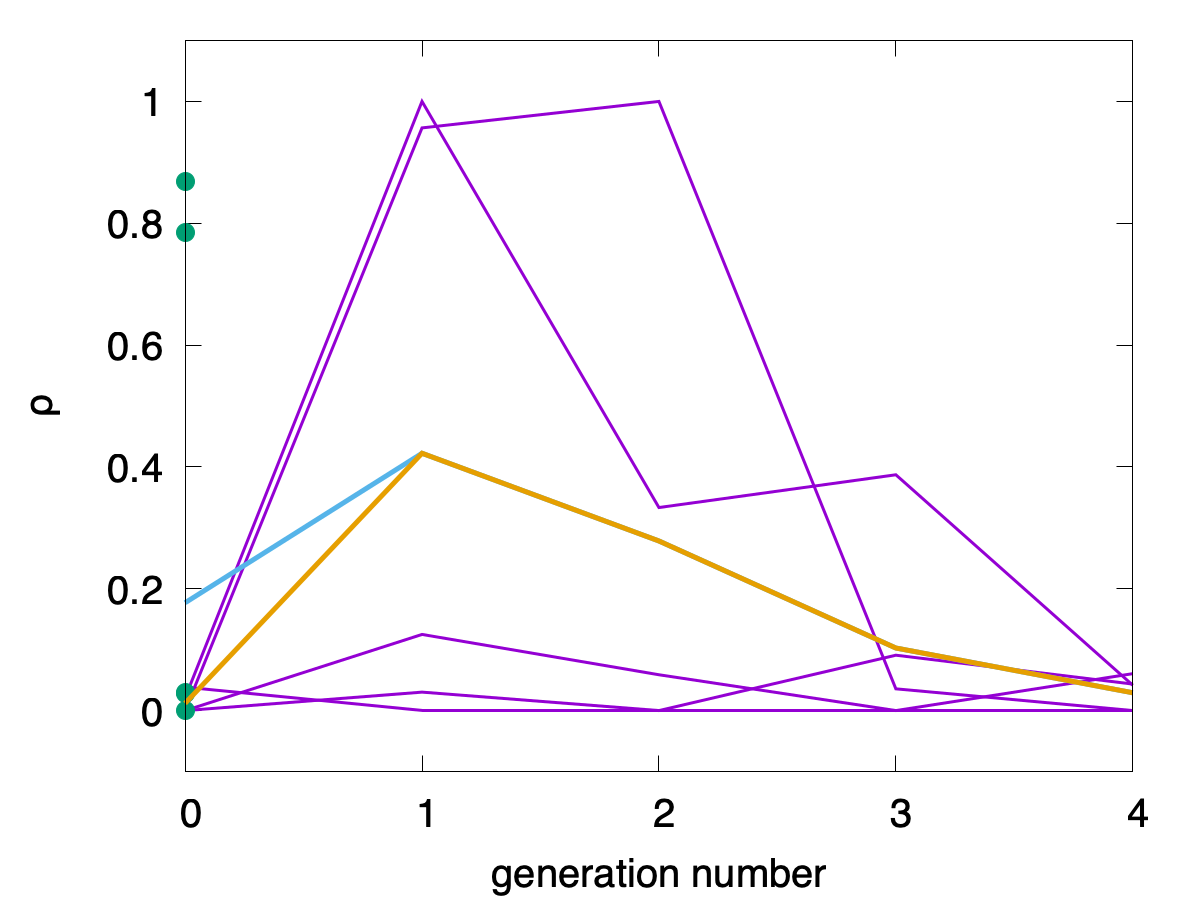
\includegraphics[width=.8\textwidth]{Pics/stats/gen-phd.png}
        \caption{} \label{fig:emma-phd-gen}
    \end{subfigure}
    \caption{$\gamma$ (a) and of $\rho$ (b) of each particle and each generation after initial selection process} 
    \label{fig:emma-gen}
\end{figure}

%%% EQUATION 
%\subsubsection{Equation}
Equations (\ref{eq:emma-phd3})-(\ref{eq:emma-vcal3}) and (\ref{eq:emma-phd4})-(\ref{eq:emma-vcal4}) represent the \gls{rf}s at $t=3$ and $t=4$, respsectively, rounded to 2 significant digits.
%$h(x)$ is the hinge function (also called a rectifier function) of the simple form $h(x) = max(0,x)$. 
The expression $h(\lambda-6)$ translates into layer count only has an influence if larger than 6 
and $h(6-\lambda)$ into layer count influential only if under 6.
%
The first thing to notice is that prediction functions of each generation depend on the same variables. 
%This means that the algorithm must decide on the variables which explain the most variance independent of optimization weights.
This stems from the fact that the algorithm choses a single minimal set of \gls{bf} to predict all dependent variables. 
%
%\td{Knowing this, makes the decision of adding $\lambda$ and $v_{cal}$ as \textit{optimizands} rather unfortunate. %highly questionable. 
%\td{This makes including $\lambda$ and $v_{cal}$ as dependent variables unfortunate decisions with hindsight.}
%As the \gls{mars} algorithm is greedy,
%Different independent variables compete to be used as \gls{bf} in the prediction functions because of the greediness of the \gls{mars} algorithm. 
%}

\begin{align}
%
%    \label{eq:emma-phd1}
%    \hat{\rho}_1 &= -26  + 0.0025 \cdot T_{DB}\cdot T{Cal}  +  0.056 \cdot  h(6-\lambda)\cdot T_{Cal} \\
%    \label{eq:emma-G1}
%    \hat{\gamma}_1 &= -0.52 + 2.3\cdot 10^{-5} \cdot  T_{DB}\cdot T_{Cal} + 0.00080 \cdot h(6-layr)\cdot T_{cal}\\
%    \label{eq:emma-layr1}
%    \hat{\lambda}_1 &= 7.1 + 8.1\cdot 10^{-5} \cdot T_{DB}\cdot T_{cal} -  0.0056 \cdot  h(6-layr)\cdot T_{cal}\\
%    \label{eq:emma-vcal1}
%    \hat{v}_{cal,1} &= 19 - 0.00025 \cdot  T_{DB}\cdot T_{cal} - 0.0055 \cdot  h(6-layr)\cdot T_{cal}\\
%
%    \label{eq:emma-phd2}
%    \hat{\rho}_2 &= 47\\
%    \label{eq:emma-G2}
%    \hat{\gamma}_2 &= 0.23\\
%    \label{eq:emma-layr2}
%    \hat{\lambda}_2 &= 7.3\\
%    \label{eq:emma-vcal2}
%    \hat{v}_{cal,2} &= 10\\
%
    \label{eq:emma-phd3}
    \hat{\rho}_3 &= 0.075  -   0.0014 \cdot  v_{cal}  +    0.18 \cdot  h(6-\lambda)  + 3.9\cdot 10^{-06} \cdot  v_{cal}\cdot T_{cal} \\
    \label{eq:emma-G3}
    \hat{\gamma}_3 &= 43  -   0.097 \cdot  v_{cal}  +     10 \cdot  h(6-\lambda)  + 0.00026 \cdot  v_{cal}\cdot T_{cal} \\
    \label{eq:emma-layr3}
    \hat{\lambda}_3 &= 9.9  - 0.00064 \cdot  v_{cal}  -     2.7 \cdot  h(6-\lambda)  - 1.3\cdot 10^{-06} \cdot  v_{cal}\cdot T_{cal} \\
    \label{eq:emma-vcal3}
    \hat{v}_{cal,3} &= -5.2\cdot 10^{-15}  +   0.016 \cdot  v_{Cal}  + 1.3\cdot 10^{-15} \cdot  h(6-\lambda)  + 3.9\cdot 10^{-21} \cdot  v_{Cal}\cdot T_{cal} \\
%
    \label{eq:emma-phd4}
    \hat{\rho}_4 &=  -0.87 + 0.0047 \cdot  T_{cal} - 0.00036 \cdot  \lambda\cdot T_{cal}  +  0.0024 \cdot  h(\lambda-6)\cdot T_{DB} \\
    \label{eq:emma-G4}
    \hat{\gamma}_4 &=     -19 + 0.28 \cdot  T_{cal}  - 0.022 \cdot  \lambda\cdot T_{cal}  +  0.16 \cdot  h(\lambda-6)\cdot T_{DB} \\
    \label{eq:emma-layr4}
    \hat{\lambda}_4 &=  6.8 - 0.014 \cdot  T_{cal}  + 0.0018 \cdot  \lambda\cdot T_{cal}  + 0.0060 \cdot  h(\lambda-6)\cdot T_{DB} \\
    \label{eq:emma-vcal4}
    \hat{v}_{cal,4} &=  29 - 0.052 \cdot  T_{cal}  + 0.0011 \cdot  \lambda\cdot T_{cal}  -  0.011 \cdot  h(\lambda-6)\cdot T_{DB} 
\end{align}

The coefficients in equations (\ref{eq:emma-phd3}) and (\ref{eq:emma-G3}) have the same signs and differ by a factor of roughly 100.
This fits the data well, but the positive influence of the layer count $\lambda$ is counter intuitive 
as one would expect more layers to be more insulating and thus result in lower conductance and a lower probability of holes going all the way trough the \gls{zro} layers. %pin hole density. 
The coefficients of the $v_{cal} \cdot T_{cal}$ interaction in equations (\ref{eq:emma-phd3}) and (\ref{eq:emma-G3}) 
seem low, but - considering the minimum value of the interaction of \num{36000} - have a higher influence on $\rho_3$ and $\gamma_3$ than the $h(6-\lambda)$ term. 
%It's positive the hinge
It is astonishing that the knot of the hinge function for equations (\ref{eq:emma-phd3})-(\ref{eq:emma-vcal3}) was chosen so low; 
basically only including the influence of $\lambda=4$.
Meaning for equations (\ref{eq:emma-phd3}) and (\ref{eq:emma-G3}) that the lowest layer count produces worse samples which is intuitive, but more than 6 layers don't improve the insulation. 
On the positive side, the calcination heating rate $v_{cal}$ (see equation (\ref{eq:emma-vcal3})) has been predicted perfectly within numerical precision. 

%%% T=4
The coefficients of equations (\ref{eq:emma-phd4}) and (\ref{eq:emma-G4}) show the same pattern 
as equations (\ref{eq:emma-phd3}) and (\ref{eq:emma-G3}): identical signs and factor 100. 
The choice of \gls{bf}s in combination with their coefficient signs seems more plausibel
for (\ref{eq:emma-phd4}) and (\ref{eq:emma-G4}) than for (\ref{eq:emma-phd3}) and (\ref{eq:emma-G3}). 
$\lambda$ decreases $\hat{\gamma}$ and $\hat{\rho}$ and additionally the lowest $\lambda$ increases the two \textit{optimizands}. 
Highly interesting is the influence of $T_{cal}$ on the measure of conductance of a sample. 
The optimzand $\hat{\gamma}$ increases with higher calcination temperature, 
ergo the resistance decreases contrary to expectations.
It was expected that 
%under \oc{400} the calcination does not fully \td{ablaufen} and 
calcination under \oc{400} does not suffice and 
that therefore the resulting layer does not insulate as well. 
Furthermore, the influence of the $T_{cal}$ term is the largest of all terms on $\hat{\rho}$ and $\hat{\gamma}$.
%This becomes clear when looking at the data.
The coefficient of the $\lambda\cdot T_{cal}$ interaction is about a tenth in size, 
but has the extra factor of $\lambda$ of up to 12, resulting in the products being in the same order of magnitude.
It can be noted that the coefficient of the $\lambda\cdot T_{cal}$ interaction always has contrary sign to $T_{cal}$ coefficient. 
This could hint a compensation of the overestimated influence of $T_{cal}$ on the \textit{optimizands}.
%It should be doubted, though, that the $layr$ only appears as interaction term 
%together with $T_{cal}$ and $T_{DB}$, which seems rather than an artefact. 
It seems rather an artefact of noise that the $\lambda$ only appears as interaction 
with $T_{cal}$ and $T_{DB}$. 

%%% MSE
For each generation the \gls{mse} was calculated for which only samples 
from the optimisation were used which were available at the time of prediction. 
That means 15 samples for $t=1$ and 30 sampes for $t=4$ were used to calculate respective \gls{mse}s. 
The \gls{mse} is 64, 158, 54 and 50 for $t=1,2,3,4$, respectively. 
It is interesting that although prediction functions for $t=3$ perfectly predicted $v_{cal}$ 
the combined \gls{mse} for $t=4$ is lower. 
The high \gls{mse} at $t=2$ can be explained by the prediction functions being only constant values. 
Apart from the second generation the \gls{mse} decreases  over time, 
which shows that the algorithm works. 
This decrease in \gls{mse} might be attributed to overfitting, though. 
%The \gls{mse} for each generation was also calculated between predicted values for pre-optimisation samples to check for overfitting, 
The \gls{mse} for each generation's prediction function was also calculated with pre-optimisation samples, which are unseen data. 
The error sank again with each generation (except for the second generation): 102, 118, 58, 50, respectively for $t=1,2,3,4$. 
%This shows 
The decrease of \gls{mse} with out-of-sample data shows that the regularization method 
of the \gls{mars} algorithm in principle works on investigated samples. 

%\td{It should be noted, that the validation \gls{mse} for $t=1$ is much higher.}
The high validation \gls{mse} (nearly 1.5 fold instead of circa 1 fold of \gls{mse}) 
for $t=1$ shows the poor prediction ability at the beginning which improved with generations.
This decrease in validation \gls{mse} supports the hypothesis stated at the beginning of this section: 
the measure of conductance was underestimated and improved over time.
%\td{why is \gls{mse} higher with higher values? No homoscedasticity ( equality of variance)?
%Or rather \gls{mse} at $t=2$ high because \gls{rf}s at $t=2$ poor and gen=2 samples are chosen with help of \gls{rf} at $t=2$? 
%}

%%% PROBLEMS 
Even though the main \textit{optimizands} were minimized as required, the \gls{rf}s were not satisfactory. 
The two main problems were too many independent variables and too many dependent variables. 
Both seem closely related and overcomplicate the optimization, but both come with their own implications. 
Too many independent variables make it harder to distinguish variance due to random error (due to unmeasured and uncontrolled variables) from variance due to dependency of chosen dependent varibales. 
This is mainly because of the curse of dimensionality\cite{friedman1988fitting} which makes it hard to collect enough data for each dimension. 
%
In the here presented optimisation model the data points per independent variable 
(events per predictor variable EPV) are as low as 5. 
By eliminating three independent variables the EVP could rise to 10, which is stated 
as rule of tumb for mulitvariate regression\cite{vittinghoff2007relaxing}. 
The results obtained with limited sample number deliver some insightfulness %are quite respectable. 
considering an EPV of 20-50 stated in the original \gls{mars} paper\cite{friedman1991multivariate} 
and an EVP of around 20 in the original \gls{emma} paper\cite{villanova2010function}. 
%In the original \gls{emma} paper\cite{villanova2010function} the EVP is 20.
%\td{In the original \gls{mars} paper\cite{friedman1991multivariate} the model is said 
%to work well on 20-50 events per predictor varibale.
%In the current model EPV are around 5, which is even low for a conservative 
%rule of thumbs of 10-15 EPV\cite{vittinghoff2007relaxing}.
%Not even rule of thumb of 10 EPV \cite{vittinghoff2007relaxing}
%Inspect \cite{friedman1988fitting,friedman1991multivariate} for further \gls{mars} discussion. 
%"The curse-of-dimensionality is fundamental and cannot be directly overcome."- Friedman 1988\cite{friedman1988fitting}.
%}
%
The main problem about too many independent variables specific to this optimisation procedure 
is that the same set of \gls{bf}s will be used to predict all \textit{optimizands}.
This leads to competition between the \gls{bf}s as not all dependent variables may depend on the same independent variables. 
This effect is reinforced by the choice of two independent variables as dependent variables. % (IVDV). 
Independent variables as dependent variables will likely be chosen in \gls{bf}s, 
for including them in the \gls{rf}s is an easy way to reduce the \gls{mse}.
These \gls{bf}s then "take away places" of \gls{bf}s predicting other dependent variables in the \gls{rf}. %\td{(cf. musical chairs)} 
This in turn can lead to wrong predictions and therefore inefficient choice of future samples. 



\td{
%%%%%%%%%%%%%%%%%%%%%%%%%%%%%%%%%%%%%%%%%%%%%%%%%%%%%%%%%%%%%%%%%%%%%%%%%%%%%%%%%%%%%%%%
\subsubsection{rational behind including $v_{cal}$ and $\lambda$ as optimizands}
The heating rate of the calcination process $v_{cal}$ and the number of layers $\lambda$ 
were included as dependent variables with the objective to maximize with a relative weight of 0.05 each.
The idea was to maximize $v_{cal}$ and minimize $\lambda$ in order to minimize the process time. 
Another thought behind including $v_{cal}$ and $\lambda$ was to test if the algorithm would correctly predict those. 
}
%
%Three major flaws behind this consideration became obvious with time: 
%
\
\ds{
(1) The true function for predicting $v_{cal}$ and $\lambda$ are $v_cal*60$ (\oc{}/\h{} instead of \oc{}/\minutes{}) and $\lambda$, respectively. 
The algorithm will tend to include those values into the prediction function for 
all dependent variables and possibly exclude others which have more influence 
on $\gamma$ and $\rho$ (see equations (\ref{eq:emma-G4})? and (\ref{eq:emma-phd4})?).
%
(2) The algorithm would be influenced by those values to choose samples, which potentially optimize $v_{cal}$ and/or $\lambda$ but not $G$ or $\rho$. 
%
(3) needlessly making the problem more complicate %, important time (around 10\% of the samples) could have been replaced with more insightful samples. 
\begin{itemize}
    \item Every output var is independent of each other, so $v_{cal}$ can act as test 
heating rate was one of the dependent variables with the intention of minimizing the variable. 
It can also be used as test to see how well the EMMA performs (or rather, more precisely MARS).
Even if it didn't influence the fit for the other splines, but it influences the choice of samples therefore it might have slowed down the process
Overall there were too many variables involved for such a small dataset
        that means that adding dependent variables influences \td{previous variables}
\end{itemize}
}
\td{look at emma papers}
\td{change G to gamma and write enr to every figure}
\td{in \cite{friedman1991multivariate} the model is said to work well on $\frac{N}{n}$ ratios (aka events per predictor varibale (EPV)) of 20-50. 
EPV is around 5 for this model.
Not even rule of thumb of 10 EPV \cite{vittinghoff2007relaxing}
Inspect \cite{friedman1988fitting,friedman1991multivariate} for further \gls{mars} discussion. 
"The curse-of-dimensionality is fundamental and cannot be directly overcome."- Friedman 1988\cite{friedman1988fitting}.
}




%%%%%%%%%%%%%%%%%%%%%%%%%%%%%%%%%%%%%%%%%%%%%%%%%%%%%%%%%%%%%%%%%%%%%%%%%%%%%%%%%%%%%%%%5
%\subsubsection{how did evolve over time?}


\iffalse
\begin{figure}
\centering
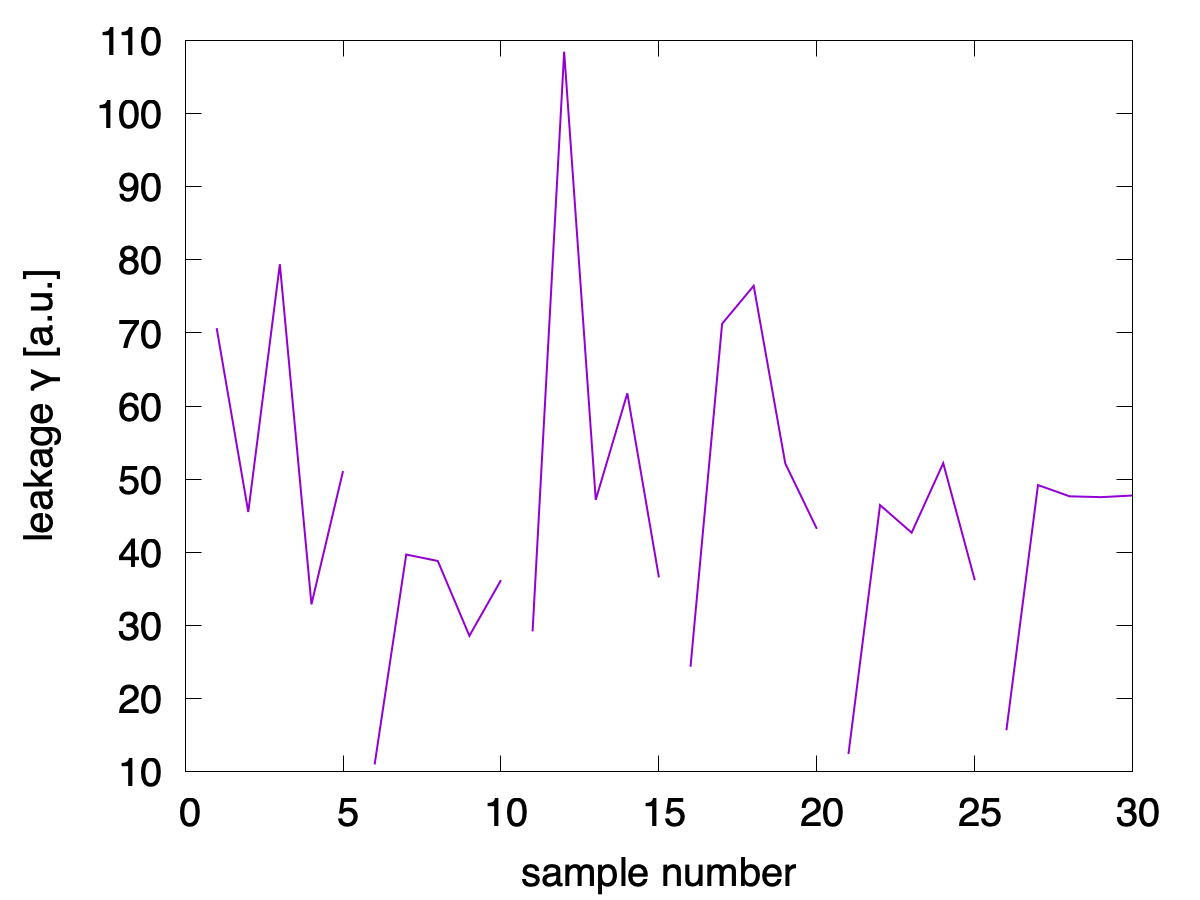
\includegraphics[width=.6\textwidth]{Pics/stats/G-t.png}
    \caption{conductivity G [a.u.] against sample number (is this even correct?)}
    \label{fig:G-t}
\end{figure}

\td{TODO: check if the sorted correctly? Make generation graph with boxplot }
\td{TODO: visualize} how the population moved across the space (with parallel coordinates? or see page 121)
\url{https://stackoverflow.com/questions/30228281/gnuplot-parallel-coordinates-axes-plot-key-annotation}
\fi

%\td{ideal objective is to create response surface approximation}\\
\td{the input vars were not regularized/normalized, naively like a small child eating old food and regretting not informing oneself earlier}\\
\td{too much data as input, dimensionality reduction (PCA) and optimization}\\
\td{pre optimization was used to check if limits where okay, but could also have been used to sieve out factors without impact on response (see miller 2001 \cite{miller2001using} section 1) }
{The primary goal of a screening experiment is to identify the active factors.
A secondary goal is to provide a simple model that captures the essential features of the 
relationship between these active factors and the response—that is, to identify the active effects. \cite{miller2001using}}

%%%%%%%%%%%%%%%%%%%%%%%%%%%%%%%%%%%%%%%%%%%%%%%%%%%%%%%%%%%
\subsubsection{diskussion and outlook}
\td{if i would plan the optimisation again, I would take less input variables (fokus on 
conc,vdoc and tdoc or even only vdoc and tdoc) which may or may not have multiple maxima.}
\td{adding a extra variable to optimize was to optimistic and ich hab mir damit eindeutig 
(im nachhinein) steine in den Weg gelegt.}
The space seems to be too big for the small sample size.
Look at relation of space size and sample size here and in Hu2016.
\td{In example of documentation 2 input variables and 1-2 responses initial population=10
, subsequent population=5, but 10 iterations. Clearly more input varibles and less 
iterations (as in actual experiments) lead to suboptimal results.
When plotting input vars  against the response variables, no trend
- The exploration-vs-exploitation parameters of the model were also not set accordingly.}
see \href{https://search.r-project.org/CRAN/refmans/emma/html/emma.html}{source}
Would be easier to fit with single factor at a time variation or latin hyper cuber? 
with same search-space to actual-data ratio
- Would it also be easier for MARS or ML to find fitting function?
plot predictions from EMMA and ML. or rather compare MAE
- the data has a lot of error, but because the production process takes so long and the 
limited time and the chosen optimisation method, the experiments weren't weiderholt
how much variance is in data? 
- The most time consuming part was definitively the prelaminary studies.
this time could have been verkürzt by testing a wide array of diverse recipes from the literature
- The data is spread across the datenraum, such that it is not trivial to 
(1) find the variable with the most variance and 
(2) to fit in order to understand to impact of noise on the data. 
- Dimension reduction bietet sich stark an bei solcher Datenlage. 
Welche methode funktioniert bei relativ vielen variablen, wenig datenpunkten und Noise. 
Am besten waere feature extraction (variable x1 hat am meisten einfluss) 
ginge auch wenn man bei pca den einfluss von verschiedenen 
I stand in front of this problem where the solution is to not use as many indep vars von vorne herein. 
- EMMA was finished on 23.02.2021 (make timeline?)
- TODO: check which software versions
-\td{for 1F c(Zr) = 44.6 mmol/L
if n is number of samples, and p is number of input variables, then n >> p 
In this case n\~50 and p\~6 which give n/p=8+1/3
in EMMA documentation example n=55and p=1-2, n/p=55-22.5
plot x vs G and hold all other vars const
write script to do that}
\todo{make sample time line with ipo vs acoh, al vs ag, hg vs doc, ...}
\td{longer literature research (first solution,second solution) and PSO wrongly eingeschaetzt, 
could have been verhindert durch lesen the docu and more papers more thoughoughly. 
Ich war geblendet von dem was ich wollte und dadurch nicht realistisch}
%\td{I-V: 2 terminal measurement one terminal was varibale and the other the ground from $-5*10^{-3}$ V to $5*10^{-3}$ V with steps of $10^{-2}$ measure current from back bone to backbone if shorted, then can measure actual resistance of layer. resistance of steel is neglectable. In order to get an impression of the quality of the layer mutliple contact (picture) are sputtered (throuhg a mask) and statistics: Two angabewerte: the weighted durchschnit and the number of pinholes, ie the number of contacts which were shorted, have an resistance below an threshold. if tunneling, iv follows powerlaw, if direct contact, iv follows linear }
- \td{I wanted to exhaust the possibilities of EA (not having enough data). i should have rather einengen the search raum as much as possible (spreading the search room too much) and then do optimisation: fix layer count to 3 fix conc to 3F and fix calc temp and rate (or only use two extreme values)}
- \td{I wanted to let the algorithm show what I already knew instead of letting my a priori knowledge constrain the model before starting.}
- factorial design (classical \gls{doe} is more robust at feature extraction for error laden data \cite{giunta2003overview}
-\td{"Similarly, it is often wise not to plan a comprehensive experiment that involves a large number of factors of interest. Such an experiment presupposes that most or all of the factors are important contributors to changes in the response variable and that they contribute jointly; i.e., that individual factor effects and their interactions are statistically significant and meaningful." - from Gunst2007}
but on the other hand: If one ain't sure a if factor is relevant, the model should be able to detect if there is a influence. - from Haertler2014?
- let's rule out different input variables: \\
does the heating temperature influence the resistance?  no \\
does the heating velocity influence the resistance?  hardly\\
do conc and layers number influence resistance? linear \\
do db velocity and db temperautre influence resistance? how\\
- somebody very wise (my superviser) once said: we need to able to predict it otherwise it is just an engineering problem \td{(look at mail)}
- "Je grösser nämlich die Anzahl freier Parameter im Modell ist, umso grösser ist der erforderliche Datenumfang und umso ungenauer wir die statistisch gewonnene Aussgae bei gleichem Datenumfang." - Gisela Härtler\cite{haertler2014statistisch}
- \td{The disadvantage of ANOVA is that information is lost because independent variables are assumed categorical even though they are ordinal}
-comparison of population size: 
\verb|see Notes/ga_from_lit_summarj.txt|
what is the minimum of population*generation and what is 10*5 

%%%%%%%%%%%%%%%%%%%%%%%%%%%%%%%%%%%%%%%%%%%%%%%%%%%%%%%%%%%%%%%%%%%%%%%%%%%%%%%%%%%%%%%%5
%%%%%%%%%%%%%%%%%%%%%%%%%%%%%%%%%%%%%%%%%%%%%%%%%%%%%%%%%%%%%%%%%%%%%%%%%%%%%%%%%%%%%%%%5
%%%%%%%%%%%%%%%%%%%%%%%%%%%%%%%%%%%%%%%%%%%%%%%%%%%%%%%%%%%%%%%%%%%%%%%%%%%%%%%%%%%%%%%%5


%%%%%%%%%%%%%%%%%%%%%%%%%%%%%%%%%%%%%%%%%%%%%%%%%%%%%%%%%%%%%%%%%%%%%%%%%%%%%%%%%%%%%%%%%%%%%
\subsubsection{Learning from Data}
General experimental procedure from Cherkassky and Mulier\cite{cherkassky1998learning}
\begin{enumerate}
	\item State the problem 
	\item Formulate the hypothesis
	\item Design the experiment/generate the data
	\item Collect the data and perform preprocessing
	\item Estimate the model 
	\item Interpret the model/draw the conclusions
\end{enumerate}
\textbf{1. Statement of the Problem} There was no clear statement of the problem. Now I would formulate it: "How to produce most insulating layer with least energy? How do we define most insulating?" That's why there are two output variables rather than one.
\textbf{2. Hypothesis Formulation} formulate an unknown dependency and define input and output variables.
\textbf{3. Data Generation and Experiment Design} can be either in control of the modeler (designed experiment) or in an observational setting. The data collection can affect the sampling distribution and influence the next steps. 
\textbf{4. Collect the Data and Perform Preprocessing} here outliers are detected and data preprocessing/encoding/feature selection. Scaling by standard deviation might be a good idea, but independent scaling of variables can lead to suboptimal representation for the learning task. Feature selection: A small number of informative features make the task of estimating dependencies easier. 
\textbf{5. Model Estimation} The main goal is to construct a model for accurate prediction of future outputs
\textbf{6. Interpret the Model and Drawing Conclusions} The interpretability and accuracy of the model are compete. In classical statistics such as linearly parametrized function will suit both requirements. More complex and flexible models might lead to better estimates with less interpretability. Identifying the most important input variables. \cite{cherkassky1998learning}

There are not only \textbf{x}(input) and y(output) variables, but also \textbf{z}(uncontrolled/unobserved input variables).
Issues of methods for learning from data: 
\begin{itemize}
	\item How to incorporate a priori assumptions into learning? 
	\item How to measure model complexity (i.e. flexibility to fit the training data)?
	\item How to find a optimal balance between the data and a priori knowledge? 
\end{itemize}
\cite{cherkassky1998learning}

"Learning is the process of estimating an unkown (input,output) dependency of structure of a system using a limit number of observations."\cite{cherkassky1998learning}

The process informal part of selection of input and output variables, data encoding/representation and incorporating a prior knowledge into the design of the learning system is often more critical for an overall success than the design of the learning machine itself.\cite{cherkassky1998learning} (page 25)

"Do not attempt to solve a specified problem by indirectly solving a harder general problem as an intermediate step."\cite{cherkassky1998learning}(p33)

"This approach works well only when the number of training samples is large relative to the (prespecified) model complexity (or the number of free parameters)".\cite{cherkassky1998learning}(p41)

Modeling bias in statistics is the discrepancy of the mismatch between parametric assumptions and the true dependency.
Modeling bias is overcome by using very flexible approximation function, with the tradeoff of more complex inductive (learning) steps. 

Any learning process requires the following(p40): 
\begin{itemize}
	\item A (wide, flexible) set of approximating functions $\mathbf{f}(\mathbf{x},\omega),\; \omega \in \Omega$
	\item A priori knowledge to impose contrains
	\item An inductive principle (what needs to be done)
		\begin{itemize}
			\item penalizeation (regularization) inductive principle
			\item early stopping rules (with ANN, difficult to control and interpret)
			\item structural risk minimization (SRM) (order according to complexity)
			\item Bayesian Inference (add subjectivity to learning machine)
			\item Minimum Description Length (MDL, cryptic complicated uninteresting)
		\end{itemize}
	\item A learning method (how does it need to be done,implementation)
\end{itemize}
\cite{cherkassky1998learning}

\textbf{Curse and Complexity of Dimensionality}
goal is to estimate function with finite samples, so it's always inaccurate (biased). 
meaning full estimate only possible with high sampling density, which is difficult for high dimensional functions.
\begin{enumerate}
	\item Sample sizes yielding the same density increse exponentially with dimension.
	\item A large radius is needed to enclose a fraction of the data points in a high-dimensional space.
	\item Almost every point is closer to an edge than to another point.
	\item Almost every point  is an outlier in its own projection.
\end{enumerate}
\textbf{Other statistics}
\begin{itemize}
    \item f-test (include to ANOVA \url{https://quantifyinghealth.com/f-statistic-in-linear-regression/})
    \item p-value: Is the probability that a data point is observed under the null hypothesis. A small value argues against the null hypothesis. 
    \item t-test: will tell you if a variable is statistically significant. 
    \item f-test: will tell you if a group of variables is jointly significant
    \item T-test (signal-noise-ratio \href{https://statisticsbyjim.com/hypothesis-testing/t-tests-1-sample-2-sample-paired-t-tests/}{(click here)}): if variable are stat. significant; 
    \item F-test (ratio of variances \href{https://statisticsbyjim.com/anova/f-tests-anova/}{click here}): if group of vars stat. sig \url{https://quantifyinghealth.com/f-statistic-in-linear-regression/}
\end{itemize}

am wichtigsten is das Ziel der untersuchung! \cite{haertler2014statistisch}
"ist das modell fraglich, sollte man die Daten so erheben, als gälte das nächst kompliziertere Modell" \cite{haertler2014statistisch}
Er könnte nun die Unterschiede zwischen den Schulen "statisteisch messen"un den Schuleinfluss in der abschliessenden Analyse "herausrechnen". \cite{haertler2014statistisch}
Eine gefährliche Fehlerquelle ist dei Erwartung eines bestimmten Ergebnisses durch den Experimentator. \cite{haertler2014statistisch}
%%%%%%%%%%%%%%%%%%%%%%%%%%%%%%%%%%%%%%%%%%%%%%%%%%%%%%%%%%%%%%%%%%%%%%%%%%%%%%%%%%%%%%%%%%%%%
\subsubsection{LINKS}
\begin{itemize}
    \item stat vs ML \url{https://medium.com/source-institute/ai-vs-statistics-c2485f9df126} and 
    \item https://towardsdatascience.com/no-machine-learning-is-not-just-glorified-statistics-26d3952234e3?gi=3f94b919de45
    \item https://towardsdatascience.com/are-you-aware-how-difficult-your-regression-problem-is-b7dae830652b calculate error/smoothness etc
\end{itemize}
%%%%%%%%%%%%%%%%%%%%%%%%%%%%%%%%%%%%%%%%%%%%%%%%%%%%%%%%%%%%%%%%%%%%%%%%%%%%%%%%%%%%%%%%%%%%%


%\clearpage

%%%%%%%%%%%%%%%%%%%%%%%%%%%%%%%%%%%%%%%%%%%%%%%%%%%%%%%
%%%%%%%%%%%%%%%%%%% 7 OUTLOOK %%%%%%%%%%%%%%%%%%%%%%%%%
%%%%%%%%%%%%%%%%%%%%%%%%%%%%%%%%%%%%%%%%%%%%%%%%%%%%%%%
\section{Outlook}
\label{sec:outlook}
%%\todo{freewriting:} 
%what did i want to do? 
The goal of this work was to find a sol-gel doctor blading process resulting in an insulating zirconium ceramic on top of steel.
This structure then can be used as substrate for thin layer photovoltaics. 
The ceramic needs to be homogeneous and defect free in order to insulate properly.
%what was done? 
A suitable recipe was found\cite{Hu2016} and the process variables were optimized via \gls{emma}. 
The recipe was improved by increasing the stability of the solution. 
The best parameters found by the \gls{emma} optimization were 
$c_{zr}=2$, $\lambda=10$, $v_{DB}=10$, $T_{DB}=40$, $v_{cal}=120$ and $T_{cal}=300$.
%\todo{$T_{cal}=300$}. 
%welche methoden wurden dafür verwendet? 
After optimization, the data was analyzed with further machine learning methods like kernel ridge regression, support vector regression and linear regression. 
The comparison of methods showed that \gls{emma} performed well on identifying the important correlation between conductance and process variables. 
%was wurde herausgefunden? 
A correlation of calcination temperature and conductance in the range of 300--500\oc{} has been detected.
Furthermore, the layer count has been verified as an important factor. 
%was kann noch herausgefundne werden und wie? 
Next steps include to investigate if the correlation of conductance and calcination temperature are statistically significant or due to small sample size. 
The aging process could be examined via infra red spectroscopy. 
%%%%%%%%%%%%%%%%%%%%%%%%%%%%%%%%%%%%%%%%%%%%%%%%%%%%%%%%%%%%%%%%%%%%%%%%%%%%%%%%%%%%%%%5
\iffalse
was kann noch veraendert werden? 
humidity 
solution age
vdb and tdb on g and phd 
Tcal on g and phd 
%%%%%%%%%%%%%%%%%%%%%%%%%%%%%%%%%%%%%%%%%%%%%%%%%%%%%%%%%%%%%%%%%%%%%%%%%%%%%%%%%%%%%%%5

Making of the solution for the sol-gel process:
For a single concentrated solution \ml{0.05} of \gls{zrpro} are added while stirring to \ml{4.95} of \gls{buoh} and stirred for \minutes{15}. 
\ml{0.013} (or one molar equvilent of Zr) of \gls{acac} is added to the stirring solution. 
After another \minutes{15} \ml{1} of acetic acid is added and stirred for \minutes{30} to stabilize the solution up to \h{24}. 

The concentration can be increased up to 5 times being stable for a minimum of \h{4}. 
The sol-gel process produces am homogeneous transparent crystalline zirconia oxide layer. 
homogeneity can be mainly controlled via blade velocity and temperature and layers can be stacked.

It should have been also verglichen with grid search with comparable size
but most time was used to find a vernuenfig base recipe and process

It is still very human 
Der process is - as it the case with all ML and most fitting processes - is very abhaengig von hyper parameters, 
In the current work population size, number of generations, and most importantly boundaries (grenzen). 
\fi

%\clearpage

\bibliographystyle{ieeetr}
\bibliography{int}

\end{document}
